% ============================================================
% CHAPITRE 6 : DEPLOIEMENT ET REALISATION
% CRISP-DM - PHASE 6 (Deployment)
% Structure canonique :
%   6.1 Planification du deploiement
%   6.2 Planification de la surveillance et de la maintenance
%   6.3 Production du rapport final
%   6.4 Revue du projet
%
% Captures : docs/rapport/img/screens/*.png (Playwright, application reelle)
% ============================================================

\chapter{Déploiement et réalisation}
\label{chap:deploiement}

% ------------------------------------------------------------
\section*{Introduction}
\addcontentsline{toc}{section}{Introduction}
% ------------------------------------------------------------

Le chapitre précédent a clos la phase d'évaluation en prononçant le passage au déploiement sous trois réserves : assistance à la décision et non automatisation, quantités recommandées présentées comme des ordres de grandeur tant que le paramétrage logistique n'est pas renseigné, et scores qualitatifs non communicables tant que la validation du juge automatique n'est pas conduite. Le présent chapitre conduit la sixième et dernière phase de CRISP-DM sous ces réserves.

C'est également le chapitre des captures d'écran. Aucune n'est apparue jusqu'ici, et ce n'est pas un effet de mise en page. Montrer l'interface avant d'avoir posé le problème, compris les données, construit les modèles et mesuré les résultats reviendrait à présenter le système par sa surface. Les écrans qui suivent ne sont pas une démonstration : ils sont la matérialisation des décisions de conception des chapitres~\ref{chap:modelisation} et~\ref{chap:evaluation}, et chacun est commenté à ce titre.

Toutes les captures présentées dans ce chapitre ont été prises sur l'application réelle, connectée à la base de production du projet et au moteur agentique en fonctionnement, au moyen d'un script d'automatisation de navigateur rejouable. Aucune n'est une maquette, aucune donnée n'y est simulée pour les besoins de l'illustration.

Le chapitre présente la stratégie de déploiement (section~\ref{sec:strategie-deploiement}), les interfaces réalisées pour le conseiller (section~\ref{sec:ui-conseiller}) puis pour le responsable (section~\ref{sec:ui-manager}), un scénario complet déroulé de bout en bout (section~\ref{sec:scenario}), le dispositif de surveillance et de maintenance (section~\ref{sec:surveillance}), et enfin la revue de projet (section~\ref{sec:revue-projet}).

% ------------------------------------------------------------
\section{Stratégie de déploiement}
\label{sec:strategie-deploiement}
% ------------------------------------------------------------

\subsection{Architecture physique}

La figure~\ref{fig:archi-physique-chap6} présente l'architecture de déploiement.

\begin{figure}[H]
    \centering
    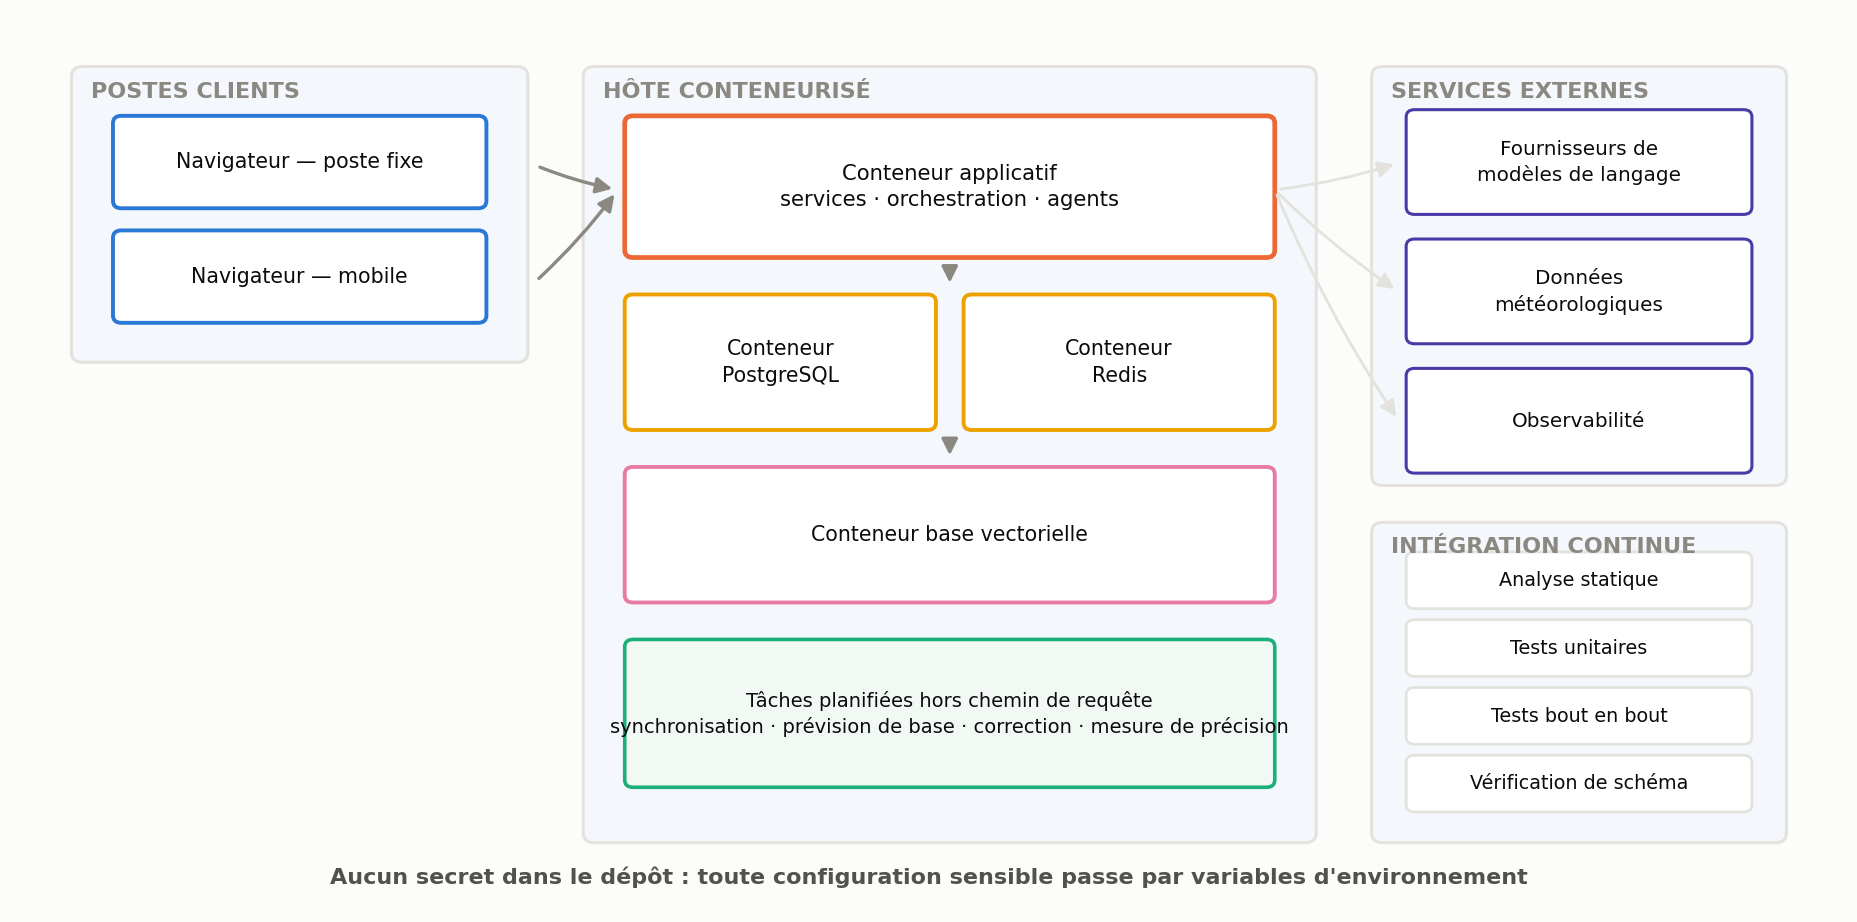
\includegraphics[width=\textwidth]{img/fig_archi_physique.png}
    \caption{Architecture physique de déploiement}
    \label{fig:archi-physique-chap6}
\end{figure}

Le déploiement repose sur la conteneurisation de chaque composant : service applicatif, base de données relationnelle, cache en mémoire, base vectorielle. Cette approche répond à une exigence identifiée au chapitre~\ref{chap:comprehension-metier} et confirmée par l'expérience du projet : la reproductibilité de l'environnement. Un projet de fin d'études destiné à être repris doit pouvoir être redémarré à l'identique par un tiers, sans reconstitution manuelle de dépendances.

Le service applicatif est déployé en processus unique exposant l'ensemble des interfaces de programmation, conformément à l'architecture monolithique modulaire retenue au chapitre~\ref{chap:modelisation}. Les traitements longs -- calcul de prévisions de base, entraînement, agrégations de grande ampleur -- sont exécutés hors du chemin de requête, par des tâches planifiées.

\subsection{Environnements et configuration}

Trois environnements sont distingués. L'environnement de \textbf{développement} fonctionne sur poste, avec des services conteneurisés locaux. L'environnement d'\textbf{intégration} est reconstruit à chaque fusion de branche par la chaîne d'intégration continue et sert à l'exécution des tests. L'environnement de \textbf{démonstration} héberge l'instance utilisée pour les captures de ce chapitre et pour la soutenance.

Aucune valeur de configuration sensible n'est inscrite dans le code : les identifiants de connexion, clés d'accès aux fournisseurs de modèles et paramètres d'environnement sont fournis par variables d'environnement. Cette règle, banale en apparence, a une conséquence directe sur la reprise du projet : le dépôt peut être partagé sans exposer aucun secret.

\subsection{Chaîne d'intégration continue et stratégie de tests}

La chaîne d'intégration continue exécute, à chaque modification, l'analyse statique, les tests unitaires du backend, les tests du frontend et les tests de bout en bout. Le tableau~\ref{tab:tests-chap6} présente la stratégie de tests.

\begingroup
\setlength{\tabcolsep}{3pt}
\renewcommand{\arraystretch}{1.15}
\small

\begin{longtable}{|P{2.8cm}|P{4.6cm}|P{6.0cm}|}
\hline
\rowcolor{red!75}
\textcolor{white}{\textbf{Niveau}} &
\textcolor{white}{\textbf{Portée}} &
\textcolor{white}{\textbf{Ce qu'il garantit}} \\
\hline
\endhead
\hline
\endfoot
\hline
\endlastfoot
Tests unitaires & Fonctions de calcul : stock de sécurité, point de commande, quantité économique, classification du risque, score produit, règles de conformité & Que les formules du chapitre~\ref{chap:modelisation} sont implémentées conformément à leur énoncé, y compris sur les cas dégénérés \\
\hline
Tests d'intégration & Chaînes agent par agent, dépôts, contrats des interfaces de programmation & Que les composants s'assemblent et que les contrats de données sont respectés \\
\hline
Tests de bout en bout & Parcours utilisateur complets sur l'application réelle & Que les parcours fonctionnent du navigateur à la base \\
\hline
Bancs d'évaluation & Six bancs du chapitre~\ref{chap:evaluation} & Que la qualité analytique ne régresse pas \\
\hline
Vérification de schéma & Cohérence entre migrations et base & Qu'aucune divergence ne s'installe entre structure voulue et structure réelle \\
\hline
\caption{Stratégie de tests par niveau}
\label{tab:tests-chap6}
\end{longtable}
\endgroup

La séparation stricte entre calcul déterministe et formulation générative, posée au chapitre~\ref{chap:modelisation}, produit ici son bénéfice le plus tangible : la totalité des calculs engageant une décision est couverte par des tests unitaires reproductibles. Une architecture où le modèle de langage aurait produit les quantités n'aurait autorisé aucune garantie de ce type.

\subsection{Contrôle d'accès}

L'authentification donne accès à un espace déterminé par le rôle et par le point de vente de rattachement. Le tableau~\ref{tab:rbac-chap6} présente la matrice d'accès effectivement appliquée.

\begingroup
\setlength{\tabcolsep}{3pt}
\renewcommand{\arraystretch}{1.15}
\small

\begin{longtable}{|P{4.4cm}|P{2.4cm}|P{2.4cm}|P{4.0cm}|}
\hline
\rowcolor{red!75}
\textcolor{white}{\textbf{Espace}} &
\textcolor{white}{\textbf{Conseiller}} &
\textcolor{white}{\textbf{Responsable}} &
\textcolor{white}{\textbf{Portée des données}} \\
\hline
\endhead
\hline
\endfoot
\hline
\endlastfoot
Mon espace & Oui & Oui & Point de vente de rattachement \\
\hline
Assistant conversationnel & Oui & Oui & Point de vente de rattachement \\
\hline
Centre de pilotage & Non & Oui & Point de vente de rattachement \\
\hline
Stock et inventaire & Non & Oui & Point de vente de rattachement \\
\hline
Arbitrage des demandes & Non & Oui & Point de vente de rattachement \\
\hline
Bons de commande & Non & Oui & Point de vente de rattachement \\
\hline
Supervision métier & Non & Oui & Point de vente de rattachement \\
\hline
\caption{Matrice de contrôle d'accès par rôle}
\label{tab:rbac-chap6}
\end{longtable}
\endgroup

Le cloisonnement s'exerce à deux niveaux : par \textbf{rôle}, qui détermine les écrans accessibles, et par \textbf{point de vente}, qui détermine les données visibles. Un conseiller ne voit ni les écrans de pilotage ni les données d'un autre point de vente. Cette double restriction est vérifiée côté serveur et non seulement par masquage d'interface.

La figure~\ref{fig:login-chap6} présente l'écran de connexion, qui distingue explicitement les deux profils.

\begin{figure}[H]
    \centering
    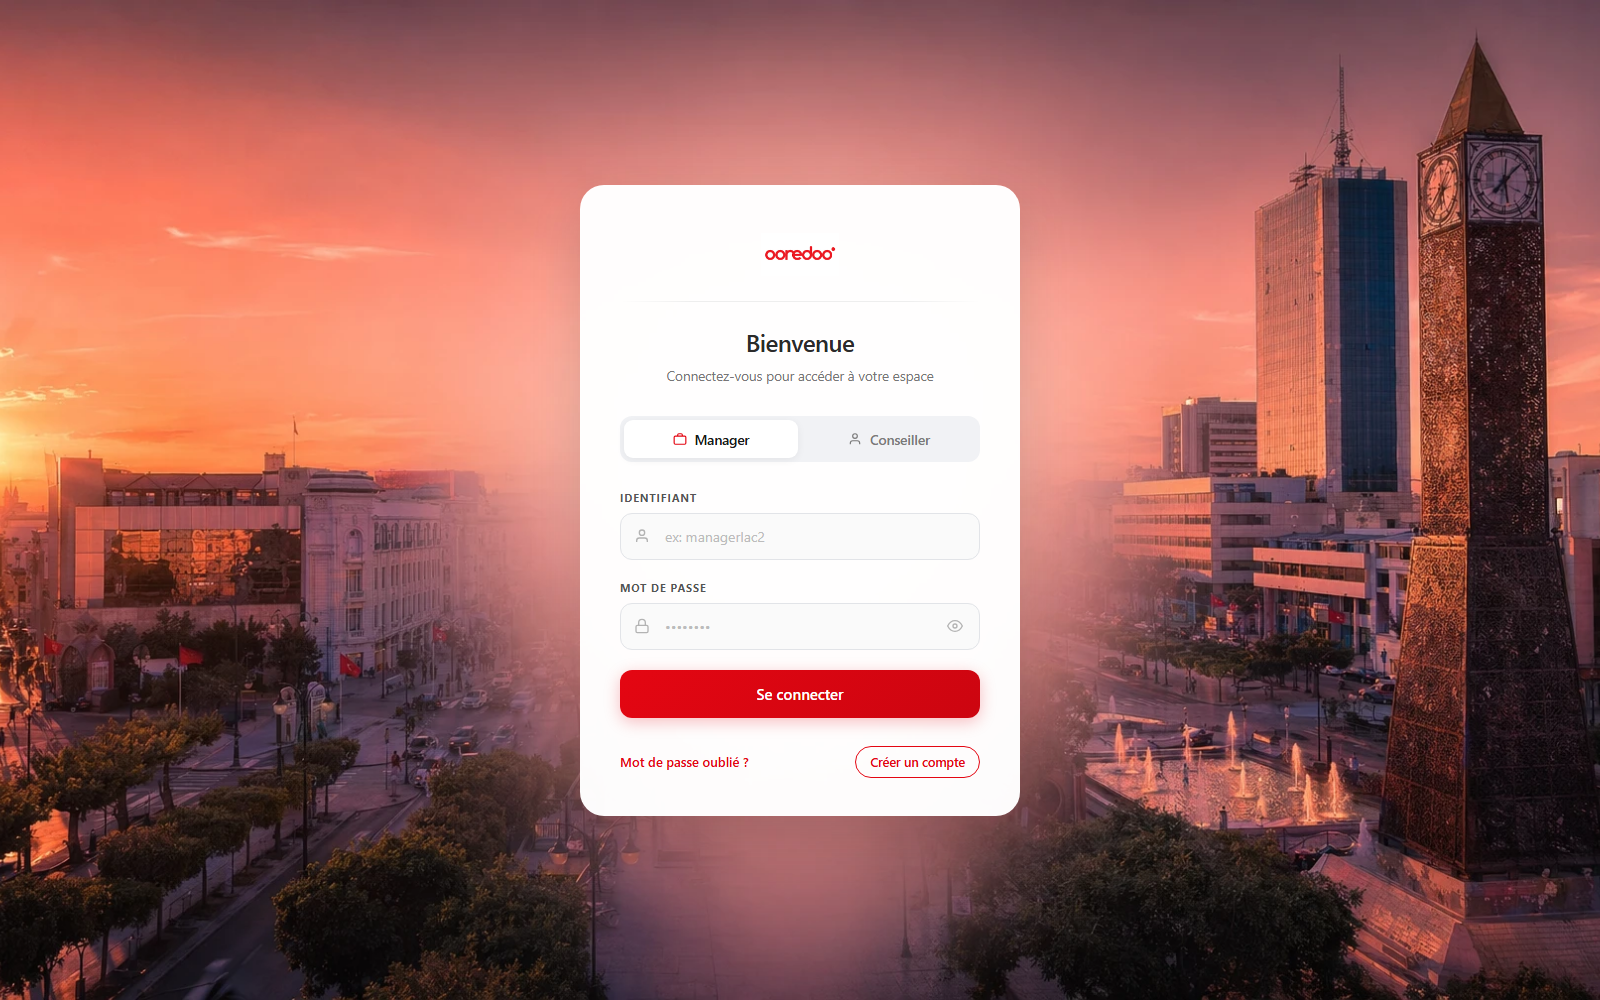
\includegraphics[width=0.72\textwidth]{img/screens/00_login.png}
    \caption{Écran de connexion : sélection du profil et authentification}
    \label{fig:login-chap6}
\end{figure}

% ------------------------------------------------------------
\section{Interfaces réalisées : espace conseiller}
\label{sec:ui-conseiller}
% ------------------------------------------------------------

\subsection{Mon espace : performance et suivi personnel}

La figure~\ref{fig:conseiller-chap6} présente l'espace du conseiller de vente.

\begin{figure}[H]
    \centering
    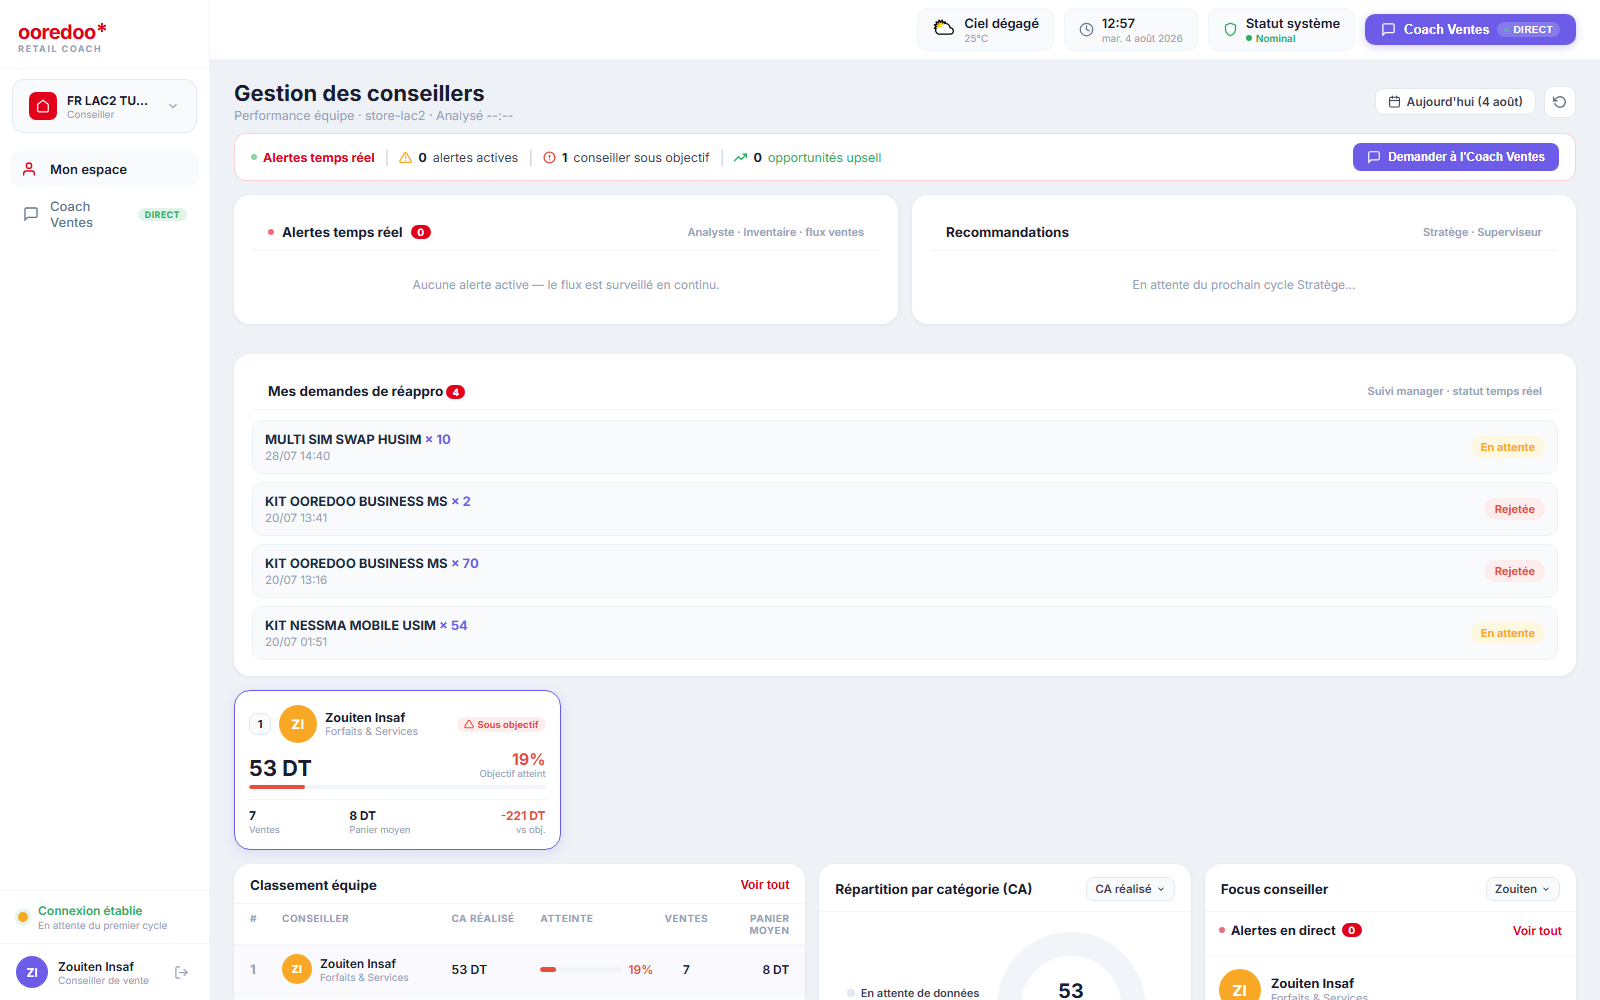
\includegraphics[width=\textwidth]{img/screens/60_conseiller_performance.png}
    \caption{Espace conseiller : performance du jour, alertes temps réel et demandes de réapprovisionnement}
    \label{fig:conseiller-chap6}
\end{figure}

Cet écran concentre ce dont le conseiller a besoin entre deux clients, dans un ordre de lecture délibéré.

En haut, une \textbf{barre d'état} indique en une ligne le nombre d'alertes actives, le nombre de conseillers sous objectif et le nombre d'opportunités identifiées. Cette synthèse est conçue pour être lisible d'un coup d'œil, sans lecture détaillée.

Au centre gauche, les \textbf{alertes temps réel} sont alimentées conjointement par l'agent Analyste, le domaine des stocks et le flux de ventes -- les trois sources sont explicitement nommées dans l'en-tête du panneau. Cette mention n'est pas décorative : elle permet au conseiller de savoir d'où vient l'information qu'il lit, exigence de traçabilité posée au chapitre~\ref{chap:comprehension-metier}.

Au centre droit, les \textbf{recommandations} du Stratège et du Superviseur. Sur la capture, le panneau affiche « En attente du prochain cycle Stratège », ce qui illustre un comportement de conception assumé : l'interface indique explicitement qu'elle attend, plutôt que d'afficher une recommandation périmée du cycle précédent. Une recommandation commerciale obsolète est plus nuisible qu'une absence de recommandation.

Le bloc \textbf{« Mes demandes de réappro »} présente les demandes émises par le conseiller et leur statut d'arbitrage par le responsable -- en attente, acceptée, rejetée. Il ferme la boucle du point de vue du conseiller : ce qu'il a demandé, ce qu'il en est advenu. Sans ce retour, le conseiller cesserait rapidement d'émettre des demandes.

En bas, la \textbf{fiche de performance individuelle} affiche le chiffre d'affaires réalisé, le taux d'atteinte de l'objectif, le nombre de ventes, le panier moyen et l'écart à l'objectif en valeur. La mention « Sous objectif » est apposée par le calcul de faisabilité du moteur de séries temporelles décrit au chapitre~\ref{chap:modelisation}, et non par une comparaison brute au prorata temporel.

\subsection{Assistant conversationnel}

Les figures~\ref{fig:chat-accueil-chap6} et~\ref{fig:chat-reponse-chap6} présentent l'assistant conversationnel.

\begin{figure}[H]
    \centering
    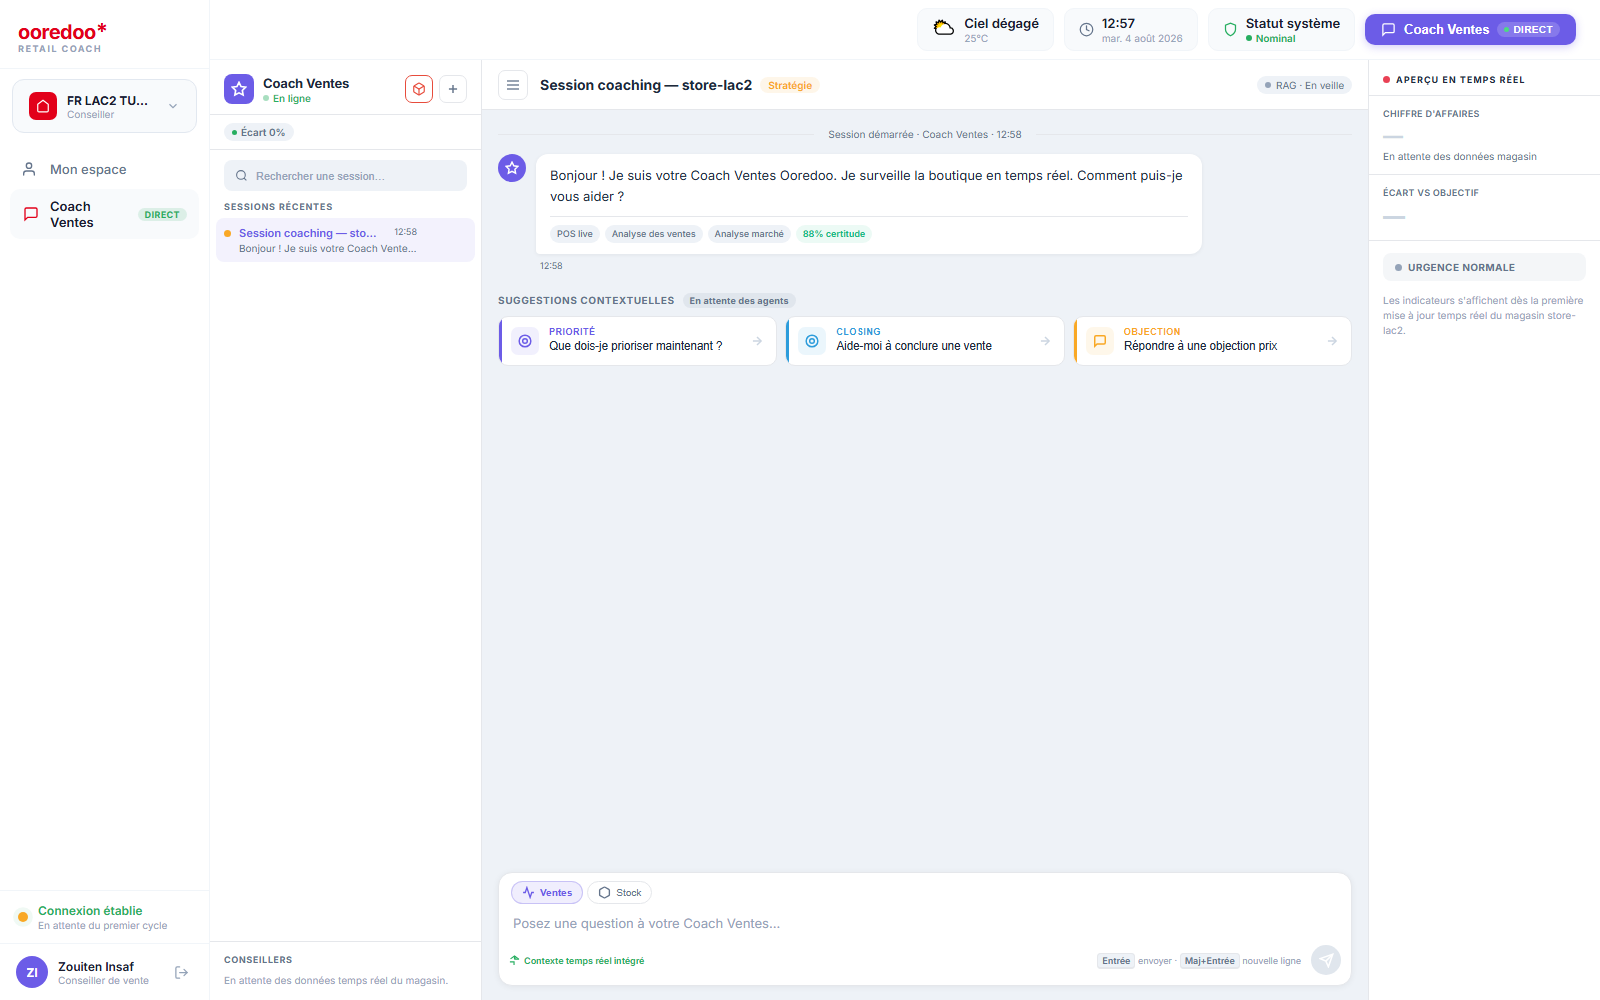
\includegraphics[width=\textwidth]{img/screens/70_chat_accueil.png}
    \caption{Assistant conversationnel : ouverture de session et contexte temps réel}
    \label{fig:chat-accueil-chap6}
\end{figure}

Trois éléments de cette interface traduisent directement des décisions de conception.

Le message d'accueil est accompagné de \textbf{marqueurs de source} -- position de caisse en direct, analyse des ventes, analyse marché -- et d'un \textbf{indice de certitude}. Le conseiller sait donc, avant même de poser sa question, sur quelles données l'assistant s'appuie et avec quel degré de confiance. C'est la matérialisation à l'écran de la hiérarchie de sources décrite au chapitre~\ref{chap:modelisation}.

Le panneau de droite, \textbf{« Aperçu en temps réel »}, affiche le chiffre d'affaires, l'écart à l'objectif et le niveau d'urgence courants. Il est alimenté par le même état partagé que les agents : l'assistant et le tableau de bord ne peuvent donc pas diverger.

Un sélecteur \textbf{« Ventes / Stock »} permet d'orienter la question vers l'un ou l'autre domaine. Il ne restreint pas la réponse mais oriente la classification d'intention décrite au chapitre~\ref{chap:modelisation}.

\begin{figure}[H]
    \centering
    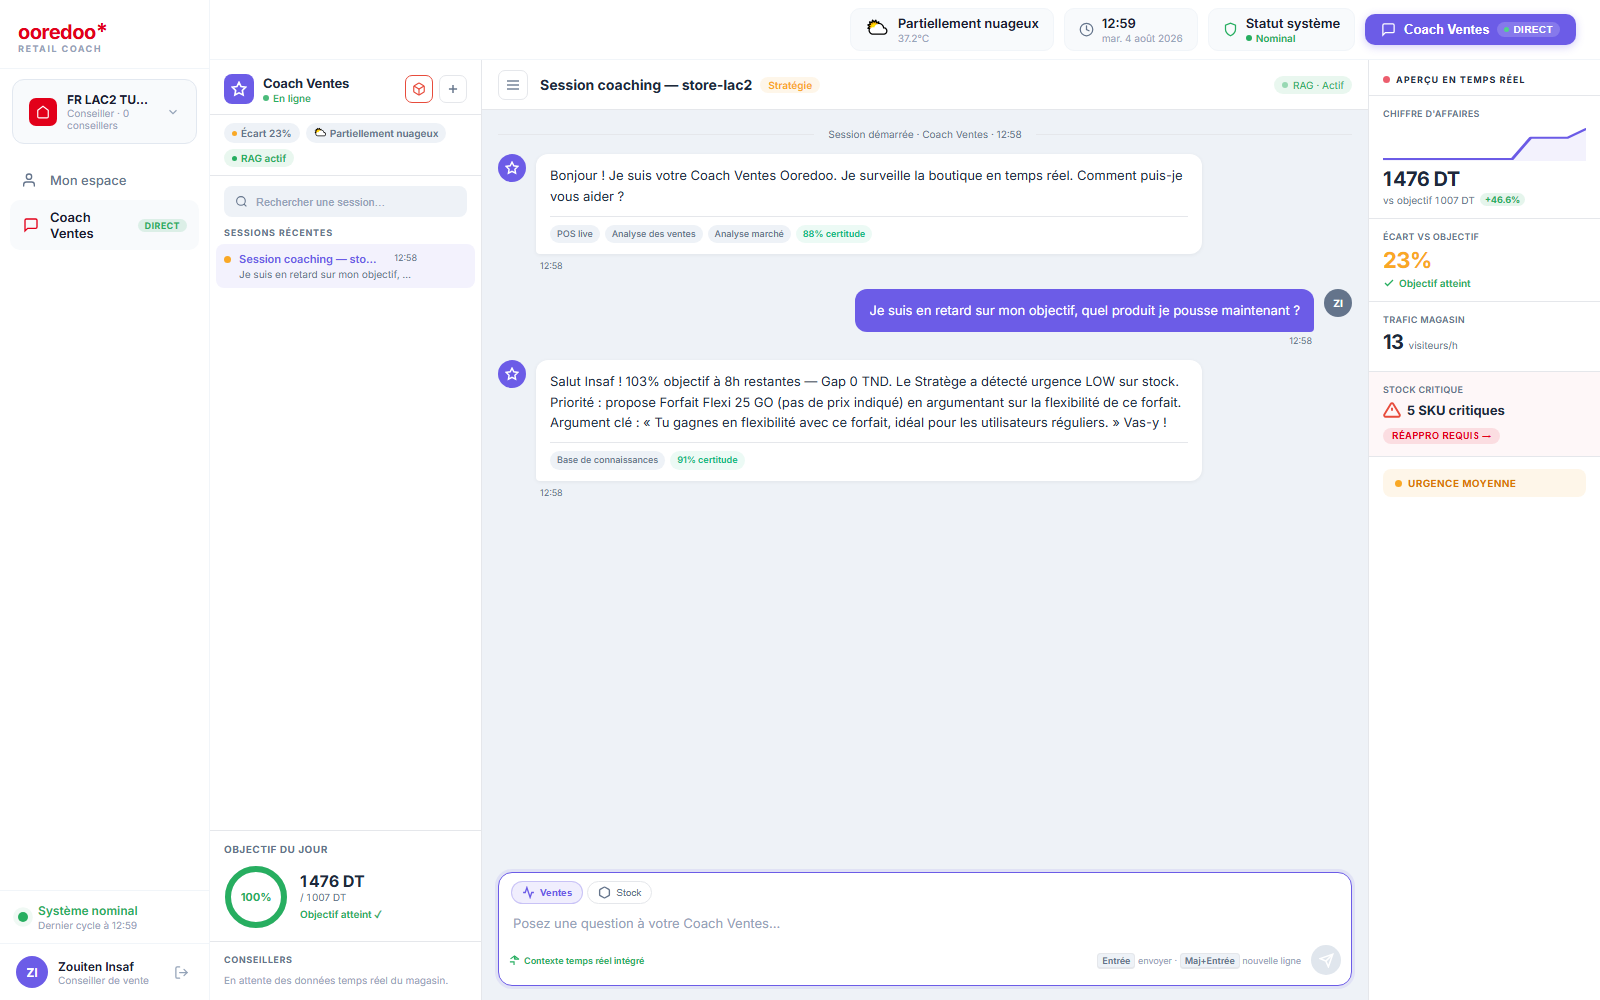
\includegraphics[width=\textwidth]{img/screens/72_chat_reponse_complete.png}
    \caption{Assistant conversationnel : réponse à une question de coaching commercial}
    \label{fig:chat-reponse-chap6}
\end{figure}

La réponse s'affiche \textbf{progressivement}, au fil de sa génération. Cette conception répond à la mesure de latence du chapitre~\ref{chap:evaluation} : avec une médiane de 6,4 secondes et un 95\textsuperscript{e} centile de 41,7 secondes, un affichage en une fois donnerait l'impression d'une interface figée. L'affichage progressif ne réduit pas la latence, il en modifie la perception -- et c'est le seul levier disponible sans dégrader la qualité.

La figure~\ref{fig:chat-substitution-chap6} illustre le mécanisme de substitution décrit au chapitre~\ref{chap:modelisation}, sollicité par une question portant sur une référence en rupture.

\begin{figure}[H]
    \centering
    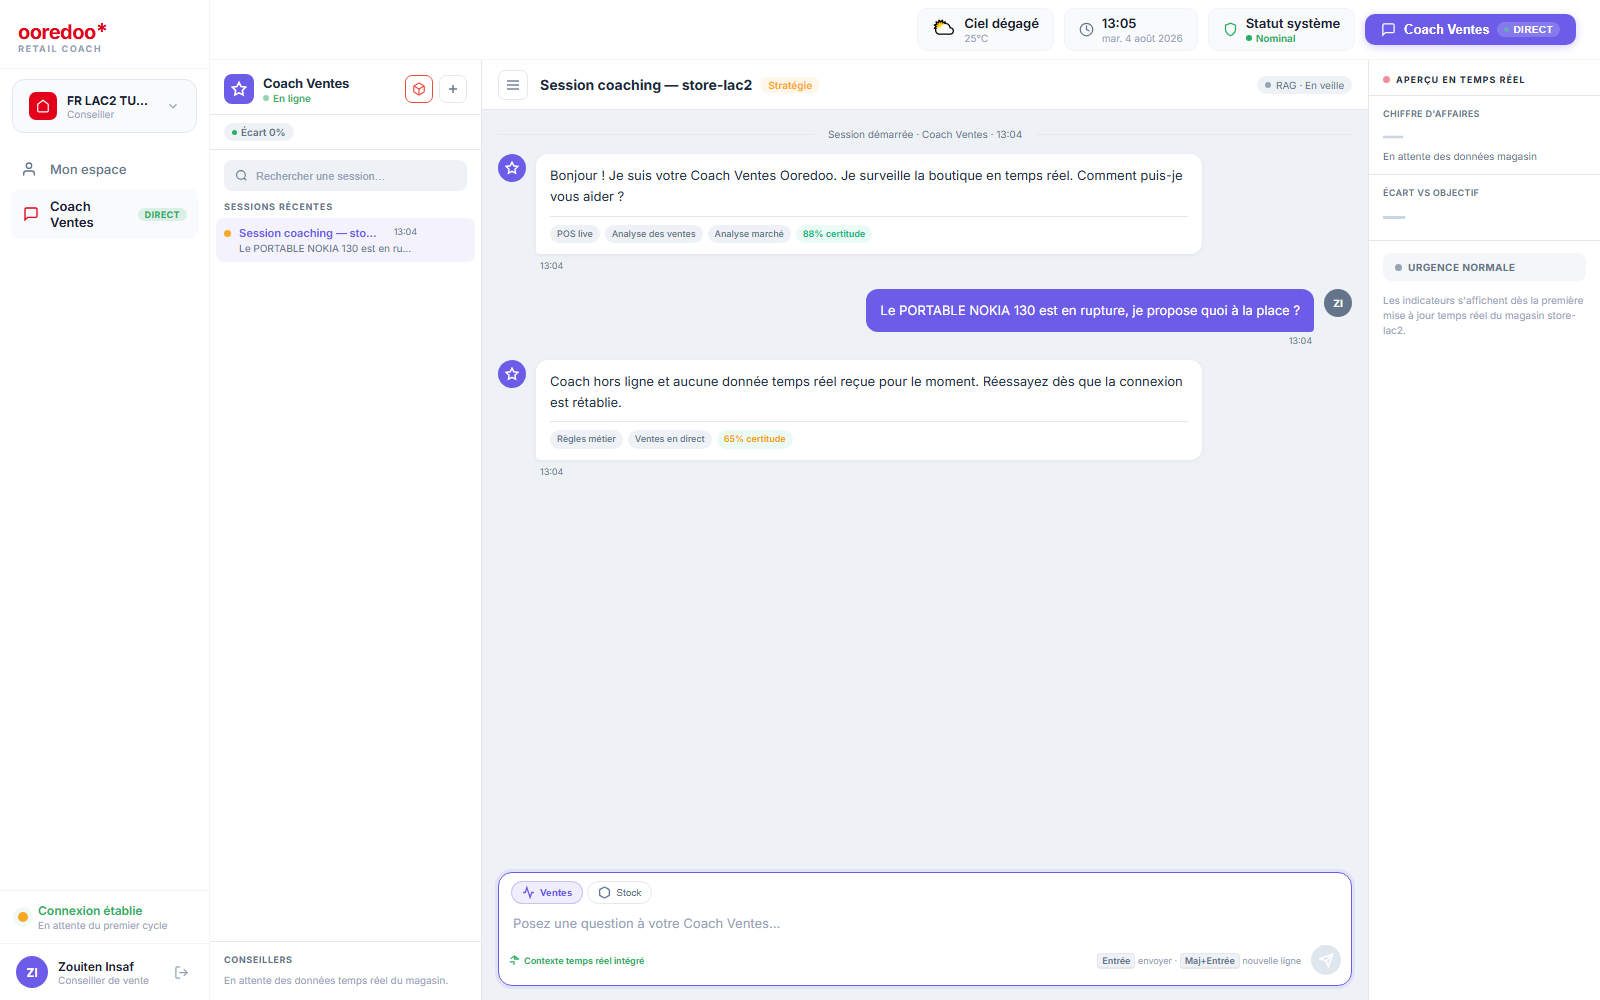
\includegraphics[width=\textwidth]{img/screens/73_chat_substitution_stock.png}
    \caption{Assistant conversationnel : substitution d'un produit en rupture}
    \label{fig:chat-substitution-chap6}
\end{figure}

C'est le croisement des deux domaines métier qui est ici visible à l'écran : la question relève de la vente, la réponse mobilise l'état du stock. Un assistant purement commercial aurait argumenté en faveur d'un produit indisponible.

\subsection{Ergonomie mobile}

Le conseiller travaille debout, souvent avec un terminal mobile. La figure~\ref{fig:mobile-chap6} présente les deux écrans principaux au format téléphone.

\begin{figure}[H]
    \centering
    \begin{minipage}{0.44\textwidth}
        \centering
        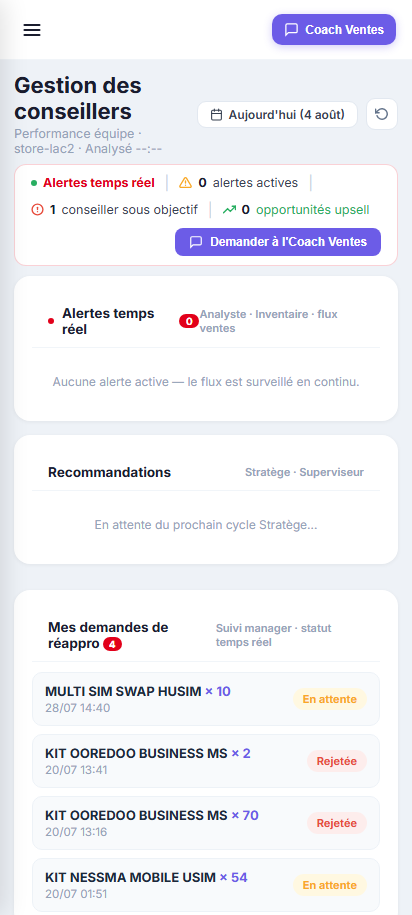
\includegraphics[width=\textwidth]{img/screens/80_mobile_conseiller.png}
    \end{minipage}\hfill
    \begin{minipage}{0.44\textwidth}
        \centering
        
\includegraphics[width=\textwidth]{img/screens/81_mobile_chat.png}
    \end{minipage}
    \caption{Adaptation au format mobile : espace conseiller et assistant conversationnel}
    \label{fig:mobile-chap6}
\end{figure}

L'adaptation n'est pas une simple réduction : la navigation latérale se replie, les tableaux deviennent des listes empilées, et les actions principales restent atteignables au pouce. L'exigence non fonctionnelle BNF-6 est ainsi satisfaite.

% ------------------------------------------------------------
\section{Interfaces réalisées : espace responsable}
\label{sec:ui-manager}
% ------------------------------------------------------------

\subsection{Centre de pilotage}

La figure~\ref{fig:dashboard-chap6} présente le centre de pilotage du point de vente.

\begin{figure}[H]
    \centering
    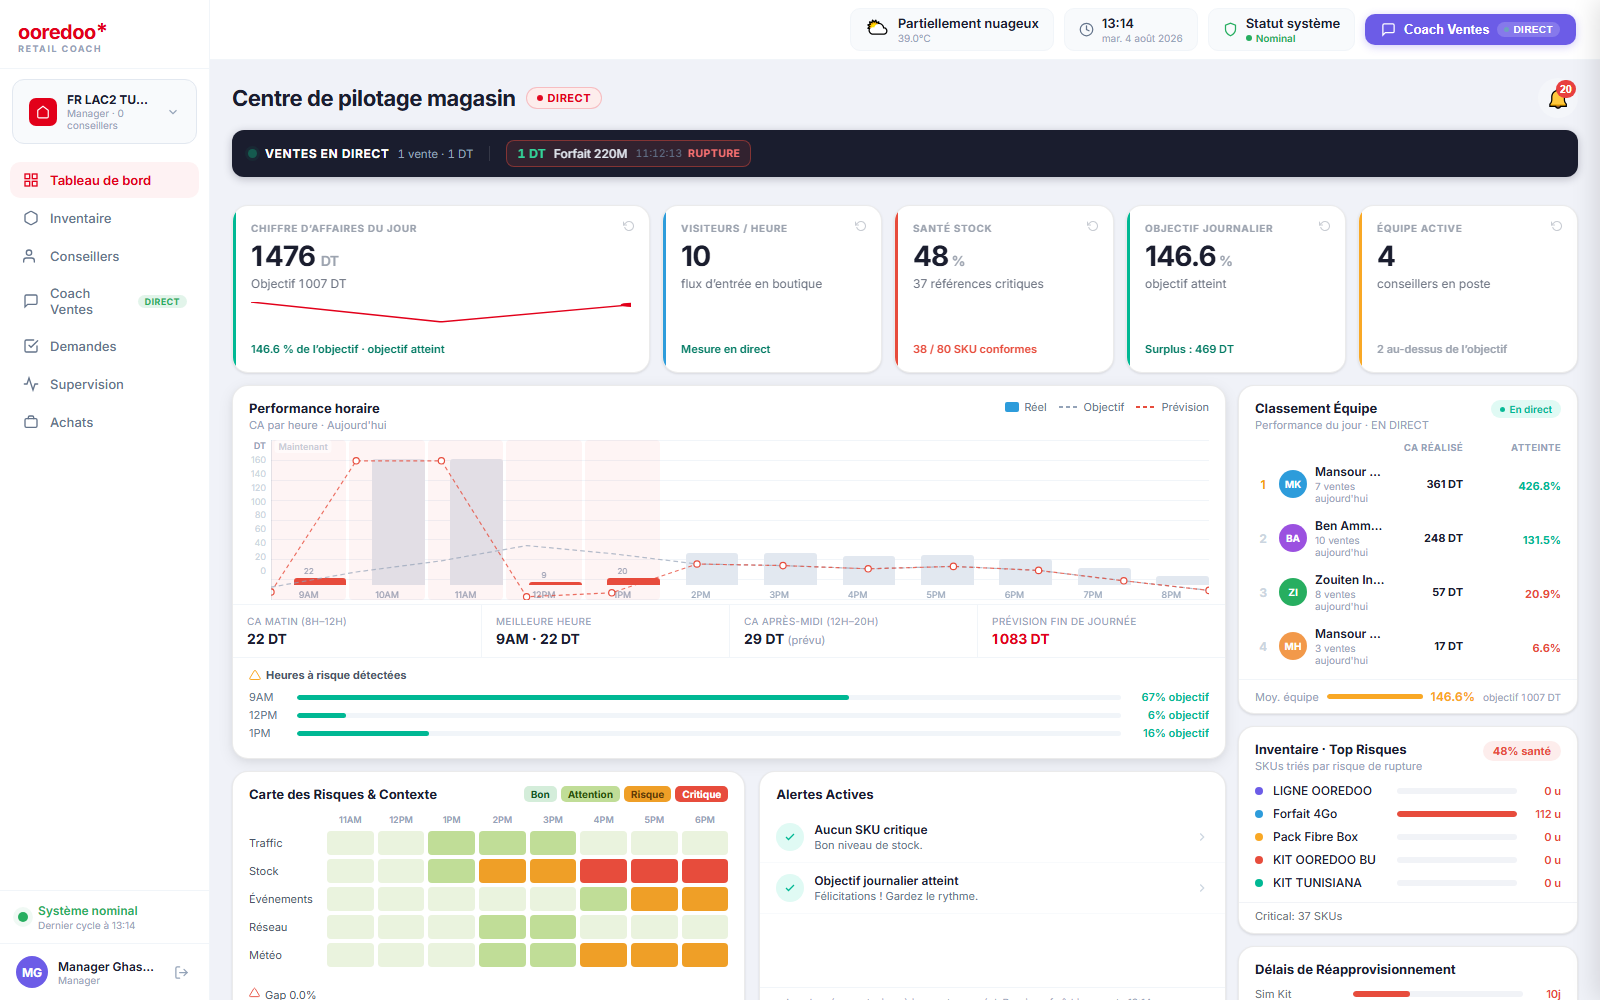
\includegraphics[width=\textwidth]{img/screens/10_dashboard_pilotage.png}
    \caption{Centre de pilotage : indicateurs, performance horaire, classement de l'équipe et carte des risques}
    \label{fig:dashboard-chap6}
\end{figure}

Cet écran rassemble cinq blocs, dont trois méritent un commentaire.

Le bandeau \textbf{« Ventes en direct »} affiche les dernières transactions à mesure qu'elles surviennent, avec l'indication de rupture lorsque le produit vendu était le dernier en stock. Il matérialise le flux temps réel décrit au chapitre~\ref{chap:donnees} et sert de preuve visible que le système est bien connecté au comptoir.

Le graphique de \textbf{performance horaire} superpose trois séries : le réalisé par heure, l'objectif proratisé et la prévision. C'est la représentation directe du moteur de séries temporelles du chapitre~\ref{chap:modelisation} : les barres portent le réalisé, la courbe pointillée porte le profil intra-journalier attendu, et la zone grisée en début de journée signale les heures écoulées avant l'ouverture effective. C'est en comparant les barres à la courbe que le responsable lit un écart horaire -- exactement la grandeur que l'objectif OD-2 formalise.

La \textbf{carte des risques et du contexte} croise cinq dimensions -- fréquentation, stock, événements, réseau, météo -- sur une échelle horaire, avec un code couleur à quatre niveaux. C'est la restitution visuelle de l'agent Contexte : chaque case indique le niveau de risque d'une dimension à une heure donnée. Cette représentation permet au responsable de comprendre \textit{pourquoi} l'après-midi est signalé comme risqué, et non seulement \textit{qu'il} l'est.

Le \textbf{classement de l'équipe} affiche, par conseiller, le chiffre d'affaires réalisé et le taux d'atteinte, actualisé en direct. Il alimente le critère de performance historique du score produit décrit au chapitre~\ref{chap:modelisation}.

Une observation d'exploitation doit être rapportée ici, par honnêteté : sur certaines captures, l'indicateur de chiffre d'affaires du jour affiche une valeur nulle alors que le bandeau des ventes en direct et le classement de l'équipe présentent des ventes du jour. Cette incohérence provient de ce que les deux blocs interrogent des sources différentes -- l'agrégat consolidé pour l'indicateur, le flux temps réel pour le bandeau -- et que la consolidation n'est pas encore effectuée à l'instant de la capture. Le défaut est identifié, son origine connue, et sa correction figure parmi les évolutions listées en section~\ref{sec:revue-projet}.

\subsection{Gestion des conseillers}

La figure~\ref{fig:equipe-chap6} présente l'écran de gestion de l'équipe.

\begin{figure}[H]
    \centering
    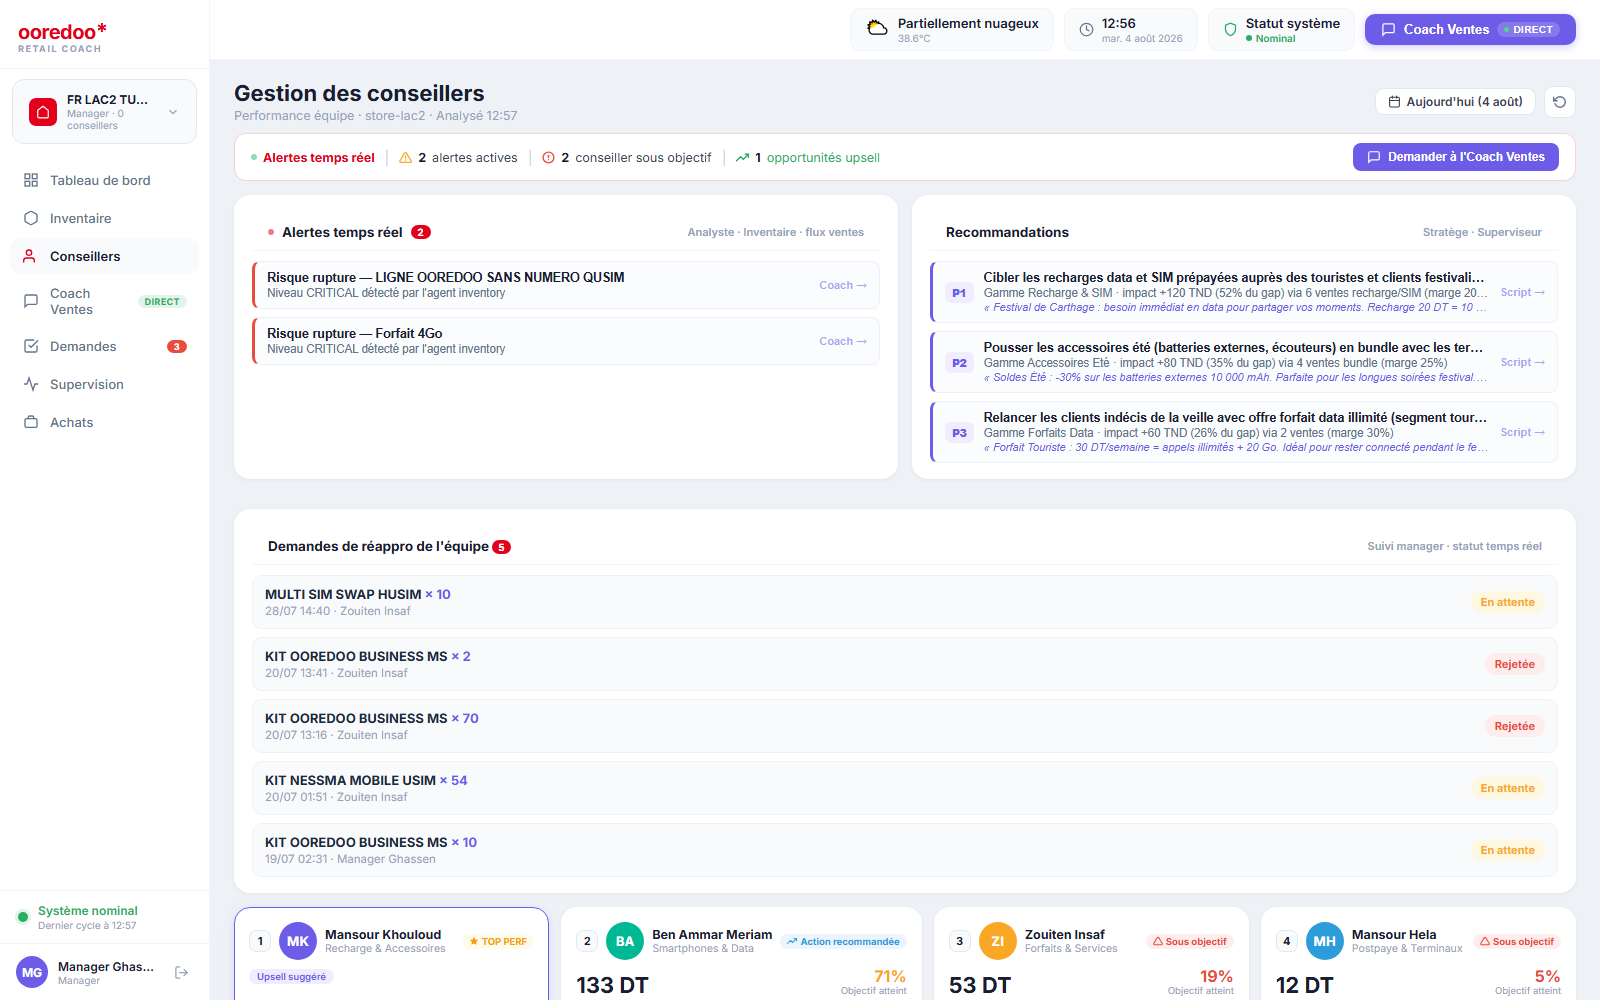
\includegraphics[width=\textwidth]{img/screens/45_conseillers_equipe.png}
    \caption{Gestion des conseillers : classement, focus individuel et répartition par catégorie}
    \label{fig:equipe-chap6}
\end{figure}

L'écran combine une vue collective -- classement, répartition du chiffre d'affaires par catégorie -- et une vue individuelle par le panneau de focus. Le passage de l'une à l'autre est ce qui rend l'écran actionnable : le classement identifie qui décroche, le focus explique pourquoi et propose l'action.

\subsection{Stock et inventaire}

La figure~\ref{fig:inventaire-chap6} présente l'écran de suivi du stock.

\begin{figure}[H]
    \centering
    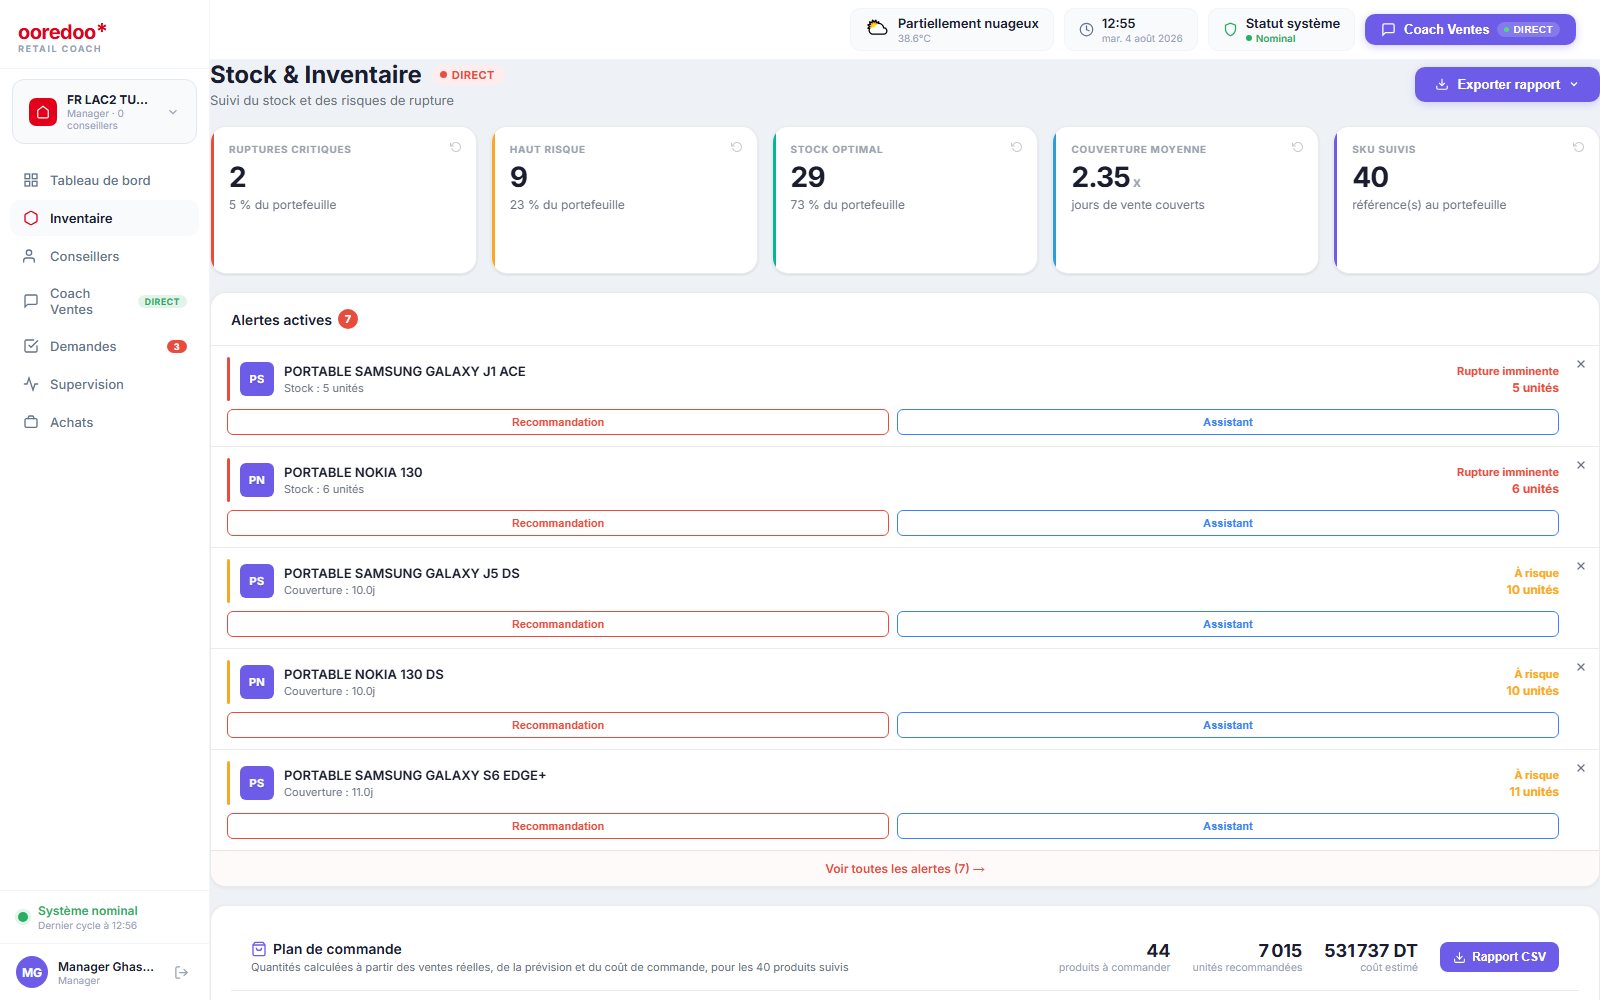
\includegraphics[width=\textwidth]{img/screens/20_inventory_portefeuille.png}
    \caption{Stock et inventaire : santé du portefeuille, alertes actives et plan de commande}
    \label{fig:inventaire-chap6}
\end{figure}

Les cinq indicateurs de tête donnent la santé du portefeuille : références en rupture critique, références à haut risque, références en stock optimal, couverture moyenne en jours de vente, nombre de références suivies. Ces valeurs sont produites par la classification à deux couches du chapitre~\ref{chap:modelisation}, et la couverture moyenne y est exprimée en jours de vente et non en unités -- seule grandeur comparable entre références.

Les \textbf{alertes actives} listent les références concernées avec leur niveau de stock et le motif du signalement. Deux actions sont proposées pour chacune : consulter la recommandation, ou interroger l'assistant à son sujet. Cette seconde action est notable : elle relie les deux espaces de l'application, permettant de passer d'un constat de stock à une conversation contextualisée sans ressaisie.

Le \textbf{plan de commande} agrège les quantités à commander sur l'ensemble du portefeuille, avec le nombre de produits concernés, le volume d'unités recommandé et le coût estimé. C'est l'agrégation des décisions individuelles de l'agent Décision. L'existence de cet agrégat répond à un besoin exprimé au chapitre~\ref{chap:comprehension-metier} : un responsable ne raisonne pas référence par référence mais par enveloppe budgétaire.

\subsection{Fiche de recommandation}

La figure~\ref{fig:reco-chap6} présente la fiche détaillée d'une recommandation de réapprovisionnement. C'est l'écran le plus important du chapitre, car il donne à voir la totalité de la chaîne de décision.

\begin{figure}[H]
    \centering
    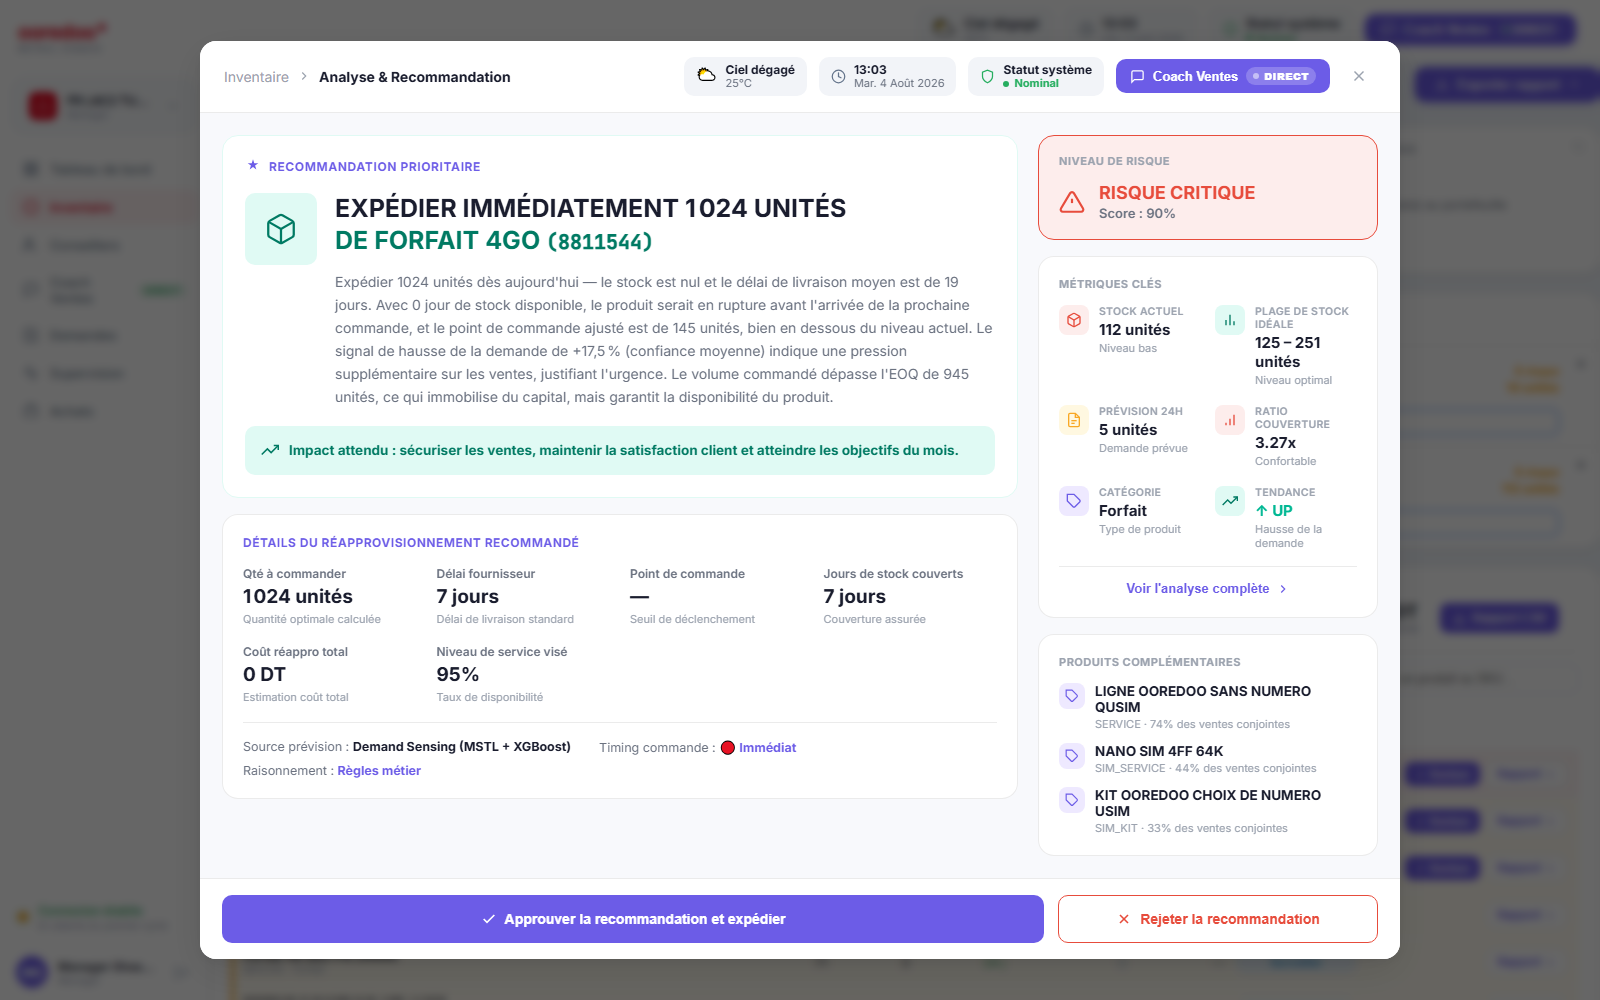
\includegraphics[width=\textwidth]{img/screens/21_inventory_fiche_reco.png}
    \caption{Fiche de recommandation : décision, justification, métriques et chaîne causale}
    \label{fig:reco-chap6}
\end{figure}

Cette fiche mérite d'être lue élément par élément, car chacun correspond à une décision de conception d'un chapitre antérieur.

L'\textbf{action et la quantité} sont annoncées en titre, sans ambiguïté. C'est la sortie de l'arbre de décision du chapitre~\ref{chap:modelisation}, ici la branche d'accélération.

La \textbf{justification} est rédigée en langage naturel et articule explicitement les grandeurs qui fondent la décision : couverture restante, délai de livraison standard, conséquence attendue, coût de l'opération, effet de la correction contextuelle avec son niveau de confiance. C'est la seule partie de la fiche produite par un modèle de langage -- et elle ne contient aucun nombre qu'il aurait calculé, tous provenant du bloc de métriques.

Le \textbf{niveau de risque} et son score proviennent de la classification à deux couches. Les \textbf{métriques clés} exposent le stock actuel, la plage de stock idéale, la prévision de demande, le ratio de couverture, la catégorie et la tendance. Le \textbf{détail du réapprovisionnement} expose la quantité, le délai fournisseur, le point de commande, les jours de couverture assurés, le coût total et le niveau de service visé.

Deux mentions de bas de fiche méritent une attention particulière, car elles relèvent de l'honnêteté du système envers son utilisateur. La mention \textbf{« Source prévision »} indique quel étage de la cascade de prévision a produit la valeur utilisée : sur cette capture, un repli de base plate, ce qui signifie que la référence ne dispose pas d'une prévision de demande complète. Le responsable sait donc que la recommandation repose sur une hypothèse dégradée. La mention \textbf{« Raisonnement »} indique si la décision provient des règles métier ou d'une évaluation générative. Ces deux mentions rendent visible, à l'écran et pour l'utilisateur final, la limite de couverture des prévisions constatée au chapitre~\ref{chap:donnees}. Un système qui les masquerait présenterait toutes ses recommandations avec la même assurance apparente, ce qui serait trompeur.

Enfin, les deux boutons d'action -- approuver et expédier, ou rejeter -- matérialisent le point d'arrêt humain. La recommandation ne devient un engagement qu'après cette décision.

\subsection{Bons de commande}

Les figures~\ref{fig:po-liste-chap6} et~\ref{fig:po-kanban-chap6} présentent le suivi des bons de commande sous ses deux vues.

\begin{figure}[H]
    \centering
    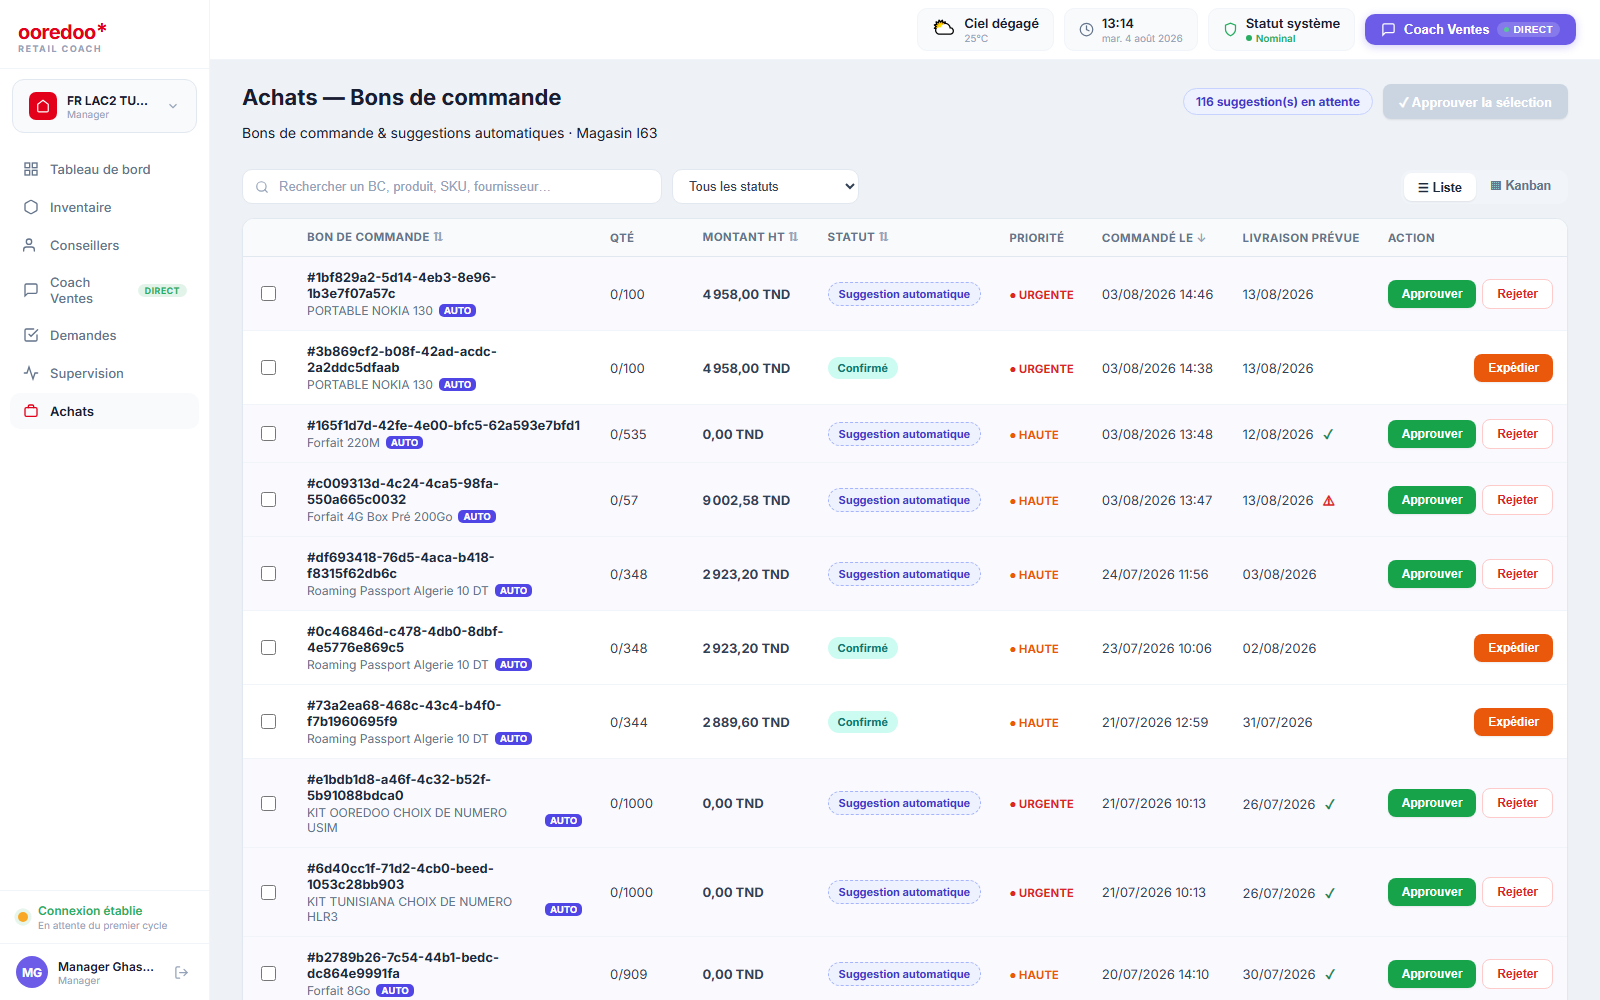
\includegraphics[width=\textwidth]{img/screens/30_purchase_liste.png}
    \caption{Bons de commande : vue liste, avec suggestions automatiques et actions d'arbitrage}
    \label{fig:po-liste-chap6}
\end{figure}

La vue liste présente chaque bon de commande avec sa quantité, son montant, son statut, sa priorité, sa date de commande et sa livraison prévue. Le marqueur \textbf{« suggestion automatique »} distingue les bons proposés par l'agent Décision de ceux créés manuellement -- distinction essentielle pour la traçabilité et pour la mesure du taux d'acceptation exploitée au chapitre~\ref{chap:evaluation}. L'indicateur de livraison signale les commandes dont la date prévue est postérieure à l'épuisement projeté du stock, ce qui déclenche l'action d'accélération plutôt qu'une nouvelle commande.

\begin{figure}[H]
    \centering
    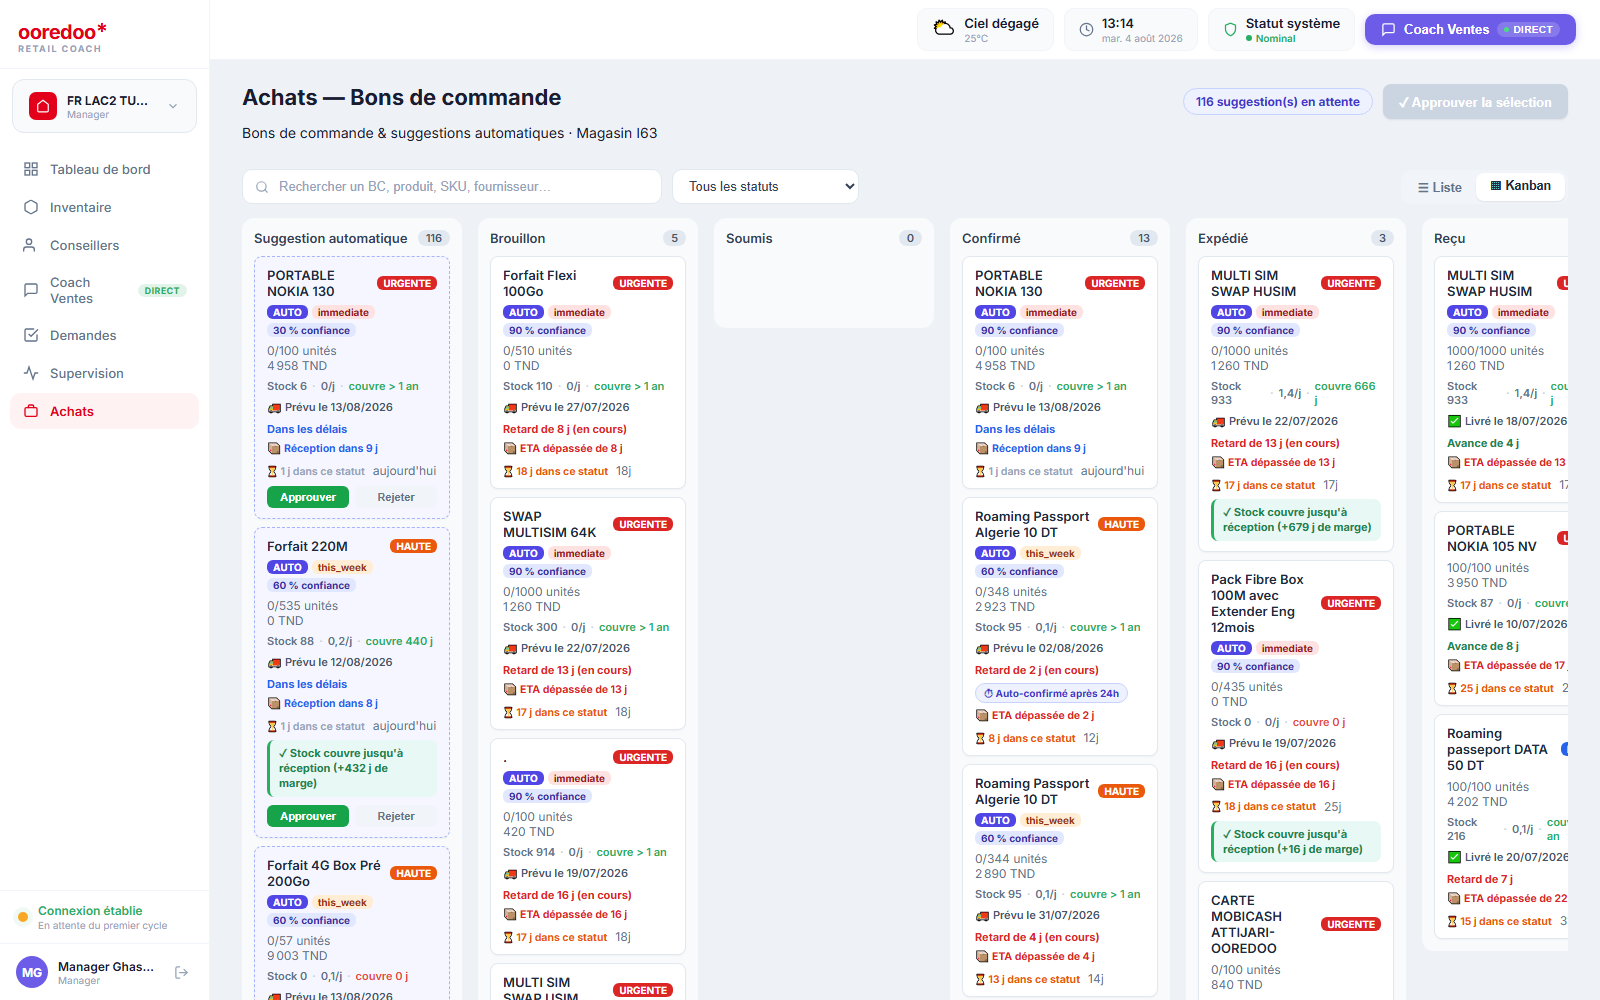
\includegraphics[width=\textwidth]{img/screens/31_purchase_kanban.png}
    \caption{Bons de commande : vue Kanban par étape du cycle de vie}
    \label{fig:po-kanban-chap6}
\end{figure}

La vue Kanban organise les mêmes bons par étape du cycle de vie défini au chapitre~\ref{chap:modelisation} : suggestion automatique, brouillon, soumis, confirmé, expédié, reçu. Elle donne au responsable la vision de flux que la vue liste ne procure pas, et elle rend immédiatement lisible la répartition de la charge entre étapes : sur la capture, la colonne des suggestions automatiques concentre l'essentiel du volume, tandis que les colonnes aval, alimentées par la seule décision humaine, en contiennent une fraction. Ce déséquilibre est la traduction visuelle du point d'arrêt humain : le système produit beaucoup de propositions, l'humain n'en retient qu'une partie.

Chaque carte porte les éléments nécessaires à l'arbitrage sans avoir à l'ouvrir : quantité reçue sur quantité commandée, montant, marqueur de suggestion automatique, indice de confiance de la recommandation d'origine, niveau de stock, couverture, date de livraison prévue, retard éventuel et ancienneté dans le statut courant. La mention indiquant si le stock couvre la période jusqu'à réception est la plus décisive : c'est elle qui distingue une commande à accélérer d'une commande qui suivra son cours.

Une fiche détaillée est accessible par ouverture d'une carte. Elle rattache le bon de commande à la recommandation qui l'a engendré -- relation ajoutée au modèle de données au chapitre~\ref{chap:donnees} -- et permet ainsi de remonter d'une commande jusqu'à l'alerte qui l'a déclenchée.

\subsection{Arbitrage des demandes de réapprovisionnement}

La figure~\ref{fig:demandes-chap6} présente l'écran d'arbitrage.

\begin{figure}[H]
    \centering
    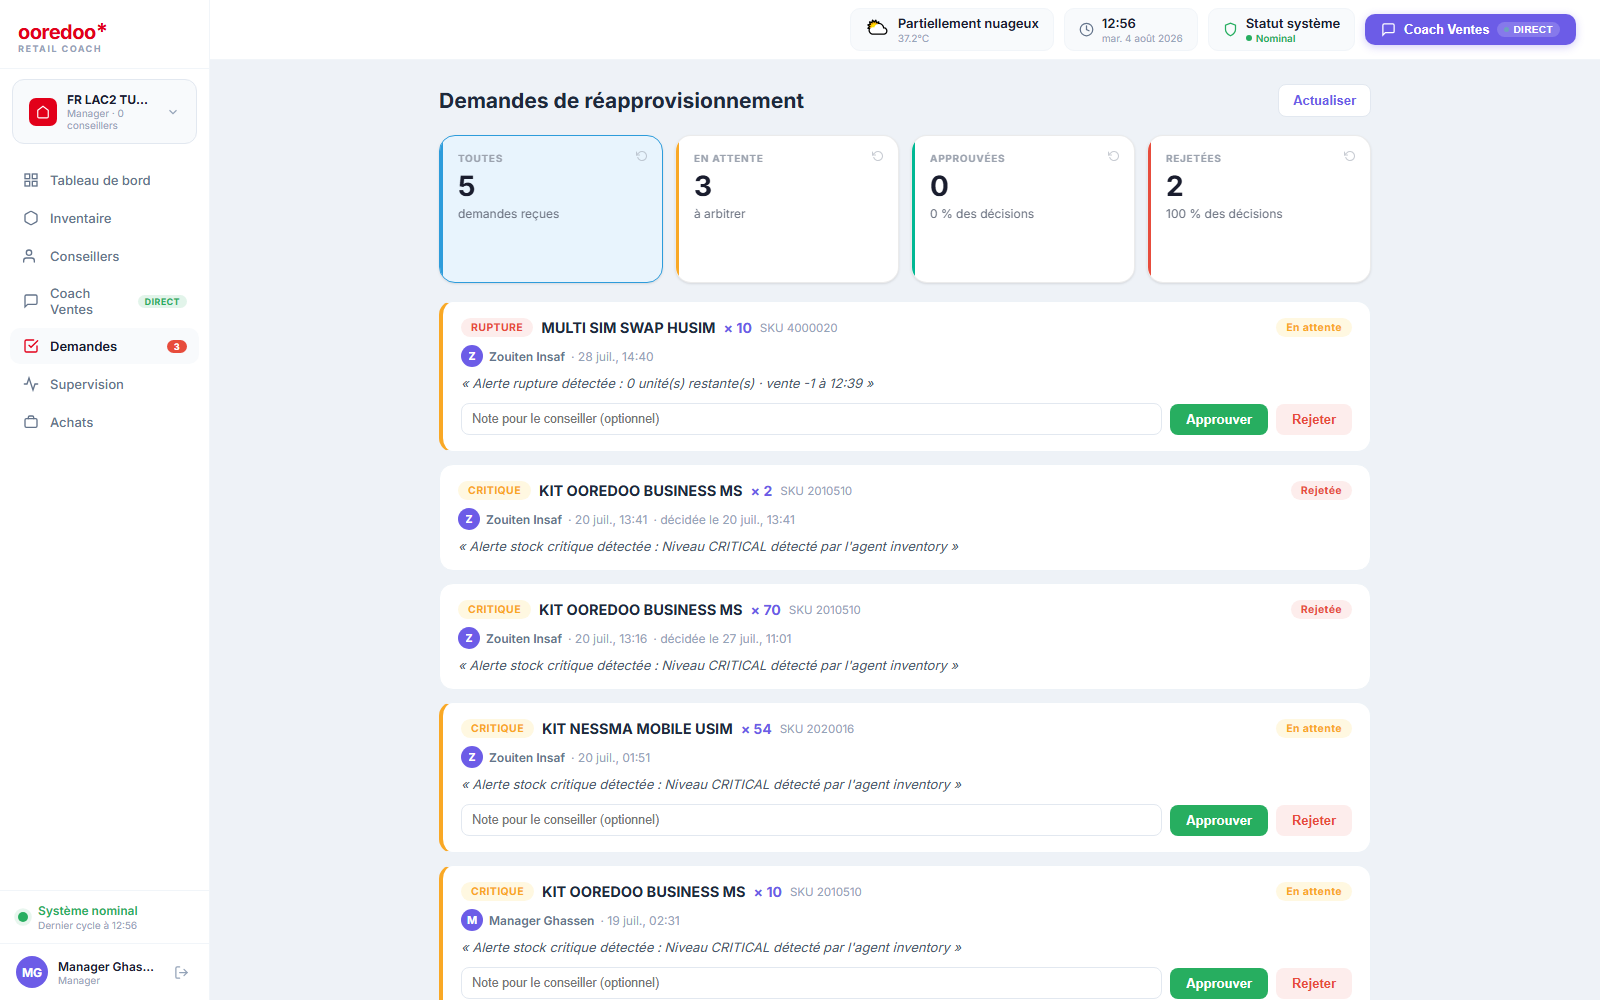
\includegraphics[width=\textwidth]{img/screens/40_demandes_arbitrage.png}
    \caption{Arbitrage des demandes de réapprovisionnement émises par les conseillers}
    \label{fig:demandes-chap6}
\end{figure}

Cet écran traite un flux distinct de celui des recommandations automatiques : les demandes émises par les conseillers depuis le terrain. Le responsable les accepte ou les rejette, et le statut est immédiatement répercuté dans l'espace du conseiller demandeur. Le motif de rejet est saisi et conservé : il alimente le dispositif d'analyse des motifs exploité au chapitre~\ref{chap:evaluation}.

\subsection{Supervision métier}

La figure~\ref{fig:supervision-chap6} présente l'écran de supervision, qui donne à voir la qualité du système lui-même.

\begin{figure}[H]
    \centering
    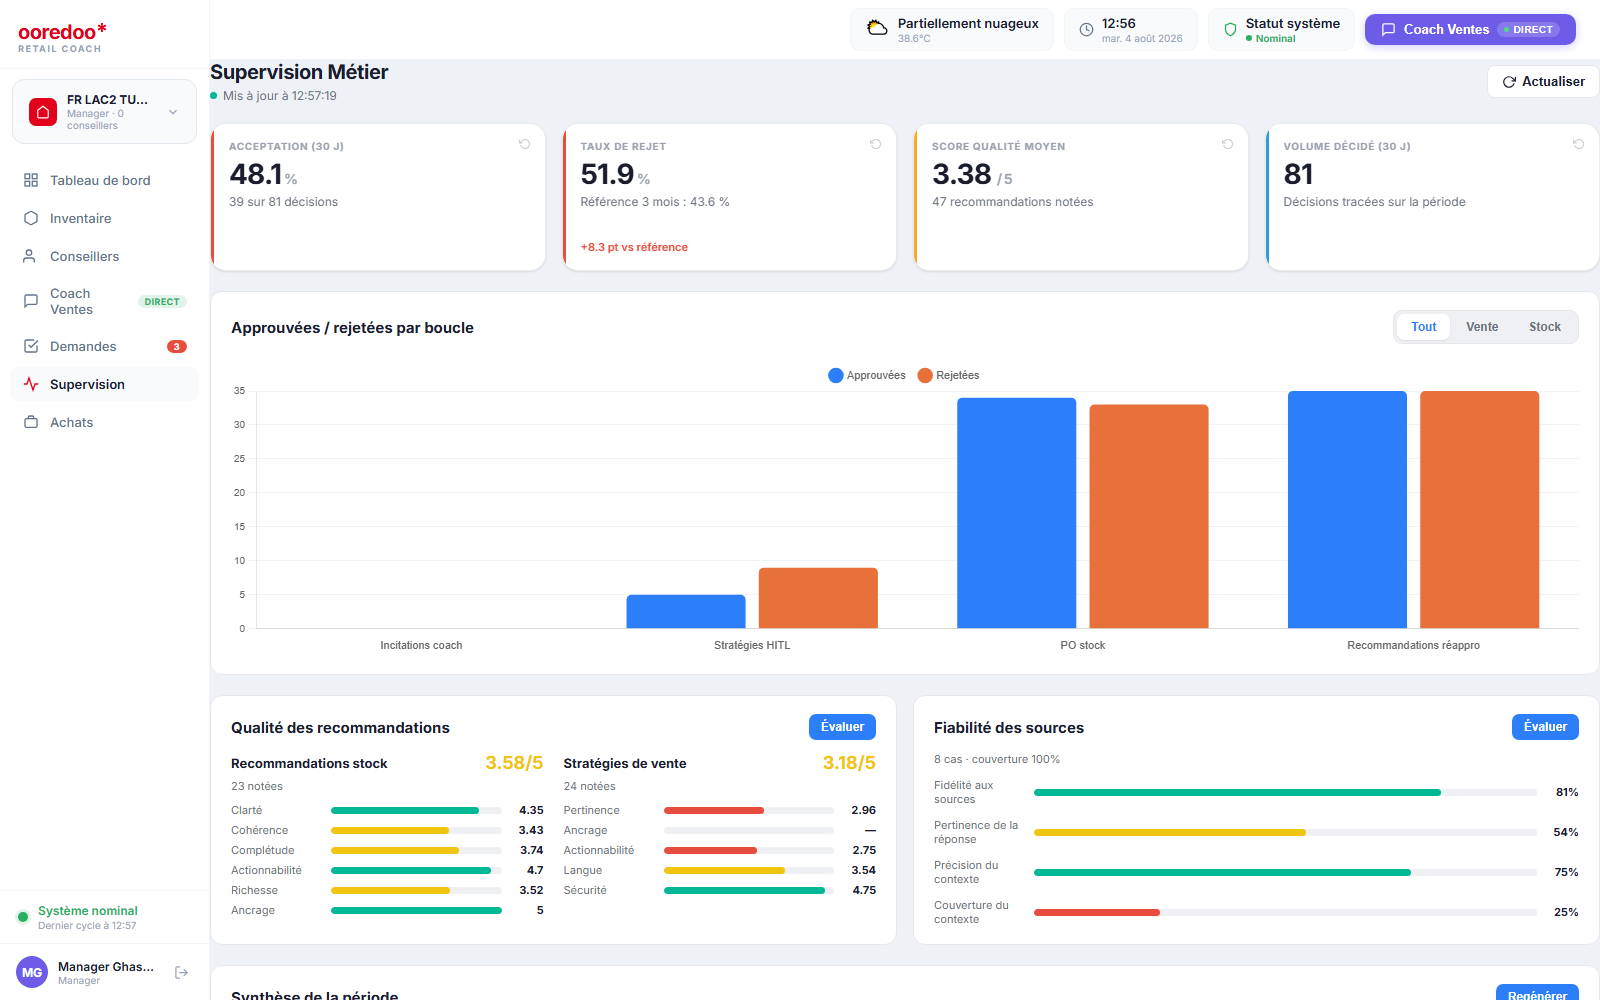
\includegraphics[width=\textwidth]{img/screens/50_monitoring_supervision.png}
    \caption{Supervision métier : acceptation, qualité des recommandations et fiabilité des sources}
    \label{fig:supervision-chap6}
\end{figure}

Cet écran est celui qui a produit une partie des mesures du chapitre~\ref{chap:evaluation}. Il n'est pas un tableau de bord technique -- durées, erreurs, consommations -- mais un tableau de bord \textbf{de qualité métier}, ce qui est nettement moins courant.

Les quatre indicateurs de tête présentent le taux d'acceptation sur trente jours, le taux de rejet avec sa comparaison à la référence des trois mois précédents, le score de qualité moyen attribué par le juge automatique, et le volume de décisions tracées. Le graphique central ventile les décisions approuvées et rejetées \textbf{par boucle de décision}, ce qui a permis d'établir au chapitre~\ref{chap:evaluation} que le déficit d'acceptation est concentré sur les stratégies commerciales et non sur les décisions de stock.

Les deux panneaux inférieurs détaillent la qualité par critère -- clarté, cohérence, complétude, actionnabilité, richesse, ancrage pour les recommandations de stock ; pertinence, ancrage, actionnabilité, langue, sécurité pour les stratégies de vente -- et la fiabilité de la chaîne documentaire. Ce sont ces valeurs qui alimentent les tableaux~\ref{tab:qualite-live-chap5} du chapitre précédent.

L'existence de cet écran est en soi un résultat du projet. Un système d'intelligence artificielle en exploitation dont personne ne mesure la qualité perçue dérive sans que quiconque s'en aperçoive. C'est cet écran qui a rendu visible l'écart de plus d'un point entre la qualité mesurée sur banc et la qualité mesurée en exploitation, résultat le plus significatif du chapitre~\ref{chap:evaluation}.

% ------------------------------------------------------------
\section{Scénario de démonstration de bout en bout}
\label{sec:scenario}
% ------------------------------------------------------------

Cette section déroule un cas complet, de la détection à la réception, en rattachant chaque étape à l'écran et au composant qui la porte. Le tableau~\ref{tab:scenario-chap6} en donne l'enchaînement.

\begingroup
\setlength{\tabcolsep}{3pt}
\renewcommand{\arraystretch}{1.15}
\small

\begin{longtable}{|P{0.9cm}|P{3.5cm}|P{4.4cm}|P{4.6cm}|}
\hline
\rowcolor{red!75}
\textcolor{white}{\textbf{Ét.}} &
\textcolor{white}{\textbf{Événement}} &
\textcolor{white}{\textbf{Composant mobilisé}} &
\textcolor{white}{\textbf{Restitution}} \\
\hline
\endhead
\hline
\endfoot
\hline
\endlastfoot
1 & Une vente épuise l'avant-dernière unité d'une référence & Flux temps réel, déclencheur sur événement de vente & Bandeau « ventes en direct » du centre de pilotage \\
\hline
2 & La couverture projetée passe sous le délai fournisseur & Agent Analyse, classification à deux couches & Alerte de rupture imminente sur l'écran d'inventaire \\
\hline
3 & L'alerte déclenche un cycle complet & Déclencheur d'alerte, graphe du superviseur & Journalisation du cycle \\
\hline
4 & Le contexte est enrichi des événements et promotions & Agent Contexte & Correction de demande appliquée \\
\hline
5 & La décision et la quantité sont calculées & Agent Décision, formules de stock & Fiche de recommandation \\
\hline
6 & La recommandation est contrôlée avant diffusion & Contrôle de conformité, 7 règles & Verdict, escalade si engagement élevé \\
\hline
7 & Le responsable approuve & Point d'arrêt humain & Bouton d'approbation de la fiche \\
\hline
8 & Un bon de commande est créé, rattaché à la recommandation & Domaine approvisionnement & Vue Kanban, colonne « approuvé » \\
\hline
9 & La commande est expédiée puis reçue & Cycle de vie du bon de commande & Progression dans le Kanban \\
\hline
10 & Le stock est mis à jour et le mouvement écrit & Dépôt d'approvisionnement & Indicateurs d'inventaire actualisés \\
\hline
11 & La décision est notée et le retour capturé & Juge en exploitation, boucle de retour & Écran de supervision métier \\
\hline
\caption{Scénario de bout en bout : de la vente à la réception}
\label{tab:scenario-chap6}
\end{longtable}
\endgroup

Ce scénario est la démonstration que la \textbf{chaîne causale est fermée}. Chaque étape est rattachée à la précédente par une relation persistée : la vente à l'alerte, l'alerte au cycle, le cycle à la recommandation, la recommandation au bon de commande, le bon de commande au mouvement de stock. C'est cette fermeture qui permet, à l'étape 11, de mesurer l'effet réel d'une décision prise à l'étape 5 -- et donc de faire progresser le système autrement que par intuition.

Il convient de rappeler que l'étape 7 n'est jamais contournée. Le système ne passe aucune commande de sa propre initiative, conformément à la première réserve du chapitre~\ref{chap:evaluation}.

% ------------------------------------------------------------
\section{Surveillance et maintenance}
\label{sec:surveillance}
% ------------------------------------------------------------

\subsection{Observabilité technique}

Chaque cycle d'agents est journalisé avec son identifiant, sa durée, les agents mobilisés, les erreurs rencontrées et le coût des appels aux modèles de langage. Cette journalisation, prévue dès la conception au chapitre~\ref{chap:modelisation}, sert deux usages : le diagnostic d'incident et le suivi du coût d'exploitation, ce dernier étant un enjeu réel dès lors que chaque cycle mobilise plusieurs appels facturés.

Un dispositif de traçage distribué permet de reconstituer le déroulement complet d'un cycle, étape par étape. Il a été déterminant lors de la résolution de plusieurs incidents rapportés en section~\ref{sec:revue-projet}.

\subsection{Suivi de la qualité en production}

Trois dispositifs fonctionnent en continu et alimentent l'écran de supervision de la figure~\ref{fig:supervision-chap6}.

La \textbf{mesure quotidienne de la précision des prévisions} confronte chaque jour la prévision de la veille aux ventes réellement observées. C'est ce dispositif qui a révélé, au chapitre~\ref{chap:evaluation}, qu'une version de modèle publiée était inopérante.

Le \textbf{juge automatique en exploitation} note en continu les productions textuelles du système sur les mêmes critères que les bancs hors ligne, permettant la comparaison directe qui a fait apparaître l'écart de plus d'un point.

La \textbf{boucle de retour humain} capture chaque approbation et chaque rejet, avec son motif.

\subsection{Plan de maintenance et de réentraînement}

Le tableau~\ref{tab:maintenance-chap6} présente le plan de maintenance.

\begingroup
\setlength{\tabcolsep}{3pt}
\renewcommand{\arraystretch}{1.15}
\small

\begin{longtable}{|P{3.6cm}|P{2.6cm}|P{6.8cm}|}
\hline
\rowcolor{red!75}
\textcolor{white}{\textbf{Opération}} &
\textcolor{white}{\textbf{Fréquence}} &
\textcolor{white}{\textbf{Déclencheur de révision}} \\
\hline
\endhead
\hline
\endfoot
\hline
\endlastfoot
Synchronisation des ventes agrégées & Quotidienne & Retard de la date la plus récente \\
\hline
Calcul de la demande de base & Tous les deux jours & Horizon de prévision insuffisant \\
\hline
Correction contextuelle & Quotidienne & Dérive de l'erreur mesurée \\
\hline
Mesure de la précision & Quotidienne & --- \\
\hline
Réentraînement du modèle de correction & À la demande & Dérive persistante de l'erreur \\
\hline
Réentraînement du modèle global de chiffre d'affaires & À la demande & Dégradation par pli, comme observée au ch.~\ref{chap:evaluation} \\
\hline
Enrichissement du corpus documentaire & Continue & Couverture de contexte insuffisante \\
\hline
Revue des règles de conformité & Trimestrielle & Apparition d'un cas non couvert \\
\hline
\caption{Plan de maintenance et de réentraînement}
\label{tab:maintenance-chap6}
\end{longtable}
\endgroup

Le réentraînement n'est volontairement \textbf{pas automatique}. Un réentraînement déclenché sans supervision peut publier un modèle dégradé sans que personne ne le constate -- exactement l'incident rapporté au chapitre~\ref{chap:evaluation}. La décision de réentraîner reste donc humaine, sur la foi de la dérive mesurée.

% ------------------------------------------------------------
\section{Revue de projet}
\label{sec:revue-projet}
% ------------------------------------------------------------

\subsection{Difficultés rencontrées et solutions apportées}

Le tableau~\ref{tab:difficultes-chap6} recense les difficultés les plus significatives et la manière dont elles ont été traitées.

\begingroup
\setlength{\tabcolsep}{3pt}
\renewcommand{\arraystretch}{1.15}
\small

\begin{longtable}{|P{3.8cm}|P{4.4cm}|P{4.8cm}|}
\hline
\rowcolor{red!75}
\textcolor{white}{\textbf{Difficulté}} &
\textcolor{white}{\textbf{Manifestation}} &
\textcolor{white}{\textbf{Solution apportée}} \\
\hline
\endhead
\hline
\endfoot
\hline
\endlastfoot
Divergence entre schéma déclaré et schéma réel & Les fichiers de migration décrivaient une structure différente de celle en production & Reconstitution d'une ligne de migrations unique et règle « aucune modification de structure à l'exécution » \\
\hline
Écritures concurrentes dans l'état partagé & Erreur d'exécution dès l'activation du parallélisme & Retour de deltas seuls, fonctions de fusion, propriété exclusive des champs \\
\hline
Corruption du stock par une suggestion & Une recommandation non approuvée augmentait le stock physique & Suppression du déclencheur fautif ; principe « une suggestion n'est pas un fait » \\
\hline
Blocage de la boucle d'événements & Interface figée pendant les calculs longs & Exécution des calculs bloquants hors de la boucle d'événements \\
\hline
Saturation des connexions à la base & Épuisement du pool sous charge & Correction d'une fuite de connexions dans la chaîne d'inventaire \\
\hline
Attributs calendaires non renseignés & Saisonnalité nulle sur toutes les références & Correction du calcul à la source, détectée par l'exploration du ch.~\ref{chap:donnees} \\
\hline
Modèle publié inopérant & Erreur de prévision voisine de 100 \% & Réentraînement sur la table de variables à jour ; détecté par la mesure quotidienne \\
\hline
Pipeline d'inventaire lent au démarrage & Première consultation de l'écran très longue & Préchauffage du cache et exécution hors chemin de requête \\
\hline
Indisponibilité de la base vectorielle & Recherche documentaire inopérante lors d'un banc & Repli lexical sur corpus local ; robustesse confirmée en conditions réelles \\
\hline
\caption{Difficultés rencontrées et solutions apportées}
\label{tab:difficultes-chap6}
\end{longtable}
\endgroup

Une lecture transversale de ce tableau est instructive. Sept des neuf difficultés relèvent de la \textbf{donnée et de l'infrastructure}, deux seulement du \textbf{modèle}. Cette répartition contredit l'intuition commune selon laquelle la difficulté d'un projet d'intelligence artificielle réside dans le choix des algorithmes. Elle rejoint en revanche ce que la littérature sur les trajectoires réelles de projets de science des données rapporte de façon constante \cite{martinez2021crisp} : la valeur se gagne et se perd dans la préparation, l'intégration et l'exploitation, bien plus que dans la modélisation.

\subsection{Écarts au plan initial}

Trois écarts au plan du chapitre~\ref{chap:comprehension-metier} doivent être signalés.

Le \textbf{périmètre de l'objectif OD-3} a été resserré aux références disposant d'un historique suffisant, décision prise en phase de compréhension des données et documentée au chapitre~\ref{chap:donnees}.

La \textbf{charge des dernières itérations} s'est révélée supérieure à la moyenne planifiée, risque identifié dès le chapitre~\ref{chap:comprehension-metier}. Les leviers d'ajustement prévus -- dépriorisation d'items secondaires et livraison en deux incréments du suivi des commandes -- ont effectivement été mobilisés.

La \textbf{validation du juge automatique}, prévue au plan, n'a pas été conduite. C'est l'écart le plus regrettable, reconnu au chapitre~\ref{chap:evaluation}.

\subsection{Perspectives d'évolution}

Les perspectives sont classées par priorité, selon leur effet attendu sur les objectifs non atteints du chapitre~\ref{chap:evaluation}.

\textbf{Priorité haute.} Conduire la validation du juge automatique, sans laquelle aucune mesure qualitative n'est probante. Enrichir le corpus documentaire, dont la faible couverture limite simultanément la pertinence du coach et la qualité de la génération ancrée -- c'est le levier unique le plus efficace sur le taux d'acceptation, qui est le critère non atteint. Renseigner les paramètres logistiques, condition pour que les quantités recommandées cessent d'être des ordres de grandeur.

\textbf{Priorité moyenne.} Corriger l'incohérence de consolidation de l'indicateur de chiffre d'affaires du jour. Abaisser le budget de latence par niveau de cascade pour ramener le 95\textsuperscript{e} centile de la réponse conversationnelle dans une plage compatible avec l'usage au comptoir. Rejouer le rétro-test de prévision avec réentraînement par pli, afin de fixer la fréquence de réentraînement.

\textbf{Priorité basse.} Étendre le périmètre à l'ensemble du réseau, l'architecture le permettant sans modification. Ajouter les fonctions classées \textit{Won't have} dans le backlog du chapitre~\ref{chap:comprehension-metier}.

% ------------------------------------------------------------
\section*{Conclusion}
\addcontentsline{toc}{section}{Conclusion}
% ------------------------------------------------------------

Ce chapitre a conduit la sixième et dernière phase de CRISP-DM. La stratégie de déploiement repose sur la conteneurisation, trois environnements distincts, une chaîne d'intégration continue exécutant cinq niveaux de tests, et un contrôle d'accès à double cloisonnement par rôle et par point de vente.

Les interfaces réalisées ont été présentées pour les deux profils d'utilisateurs. Chaque écran a été rattaché aux décisions de conception qui le fondent, plutôt que décrit pour lui-même. Deux écrans concentrent l'essentiel de l'apport du projet : la fiche de recommandation, qui expose la totalité de la chaîne de décision -- action, justification, métriques, source de la prévision, nature du raisonnement, et point d'arrêt humain --, et l'écran de supervision métier, qui mesure en continu la qualité perçue du système et a rendu visible l'écart entre performance de banc et performance réelle.

Le scénario de bout en bout a établi que la chaîne causale est fermée, de la vente qui épuise le stock jusqu'à la réception de la commande qui le reconstitue, en passant par le point d'arrêt humain qui n'est jamais contourné. Le dispositif de surveillance mesure quotidiennement la précision des prévisions, la qualité des productions textuelles et le retour humain, et le plan de maintenance conserve délibérément la décision de réentraînement à la main de l'humain.

La revue de projet a recensé neuf difficultés majeures, dont sept relèvent de la donnée et de l'infrastructure et deux seulement de la modélisation -- répartition qui constitue peut-être l'enseignement le plus durable de ce travail. Les perspectives d'évolution ont été hiérarchisées selon leur effet attendu sur le seul critère métier non atteint, l'utilité perçue des propositions.

Le cycle CRISP-DM est ainsi parcouru dans son intégralité, chaque phase ayant été close par une décision explicite autorisant la suivante. La conclusion générale qui suit dresse le bilan de l'ensemble et en tire les enseignements.
